\documentclass[a4paper, 12pt, svgnames]{article}

\usepackage{preambule}
\newcommand{\mr}[1]{{\textcolor[rgb]{0.80,0.10,0.1}{#1}}}

\title{Variabilités intrinsèques des SNe Ia et leurs conséquences sur les
paramètres cosmologiques}

\fancyhead[L]{\scriptsize \textsc{Variabilités intrinsèques des SNe Ia}}

\begin{document}

\thispagestyle{empty}
\noindent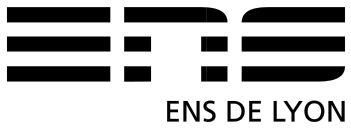
\includegraphics[height=2cm]{General_figures/logoens.png} \hfill

\includegraphics[height=2cm]{General_figures/logoucbl.png} \hfill

\includegraphics[height=2cm]{General_figures/logounivlyon.png}\vfill

\noindent\begin{tabularx}{\linewidth+27pt}{@{} l X r @{} }
{\textsc{Master Science de la matière}} & & Année 2018--2019\hspace*{1cm}\\
{\textit{École Normale Supérieure de Lyon}} & & \textsc{Nicolas} Nora\hspace*{1cm}\\
{\textit{Université Claude Bernard Lyon I}} & & M2 Physique\hspace*{1cm}
\end{tabularx}

\begin{center}\vfill\hrule\vspace*{8pt}

\textbf{\huge Variabilités intrinsèques des SNe Ia et leurs conséquences sur les
paramètres cosmologiques}\\

\hrule\vfill

\parbox{15cm}{\small\textbf{Résumé}:
L'étude des supernovae de type Ia a de nombreuses utilités en physique. Elle
sert notamment à la détermination de paramètres cosmologiques, comme la
constante de Hubble ou le paramètre d'état de l'énergie noire. Afin d'améliorer
la précision et la justesse des mesures existantes, les incertitudes
statistiques et systématiques doivent être traitées correctement. Si l'ajout de
données permet de réduire les incertitudes statistiques, il n'y a que l'étude du
comportement physique des supernovae qui permet de réduire les incertitudes
systématiques. Dans ce rapport, nous discutons comment l'établissement de lois
d'évolution du paramètre de durée d'explosion d'une supernova en fonction du
redshift permettrait d'atteindre ce but.}\vspace{0.5cm}

\parbox{15cm}{\small\textbf{Mots-clés}:
Cosmologie, supernovae}\vspace{0.5cm}

\parbox{15cm}{Stage supervisé par:\\
\textbf{\textsc{RIGAULT} Mickaël}, Chercheur\\
\href{mailto:rigault@ipnl.in2p3.fr}{rigault@ipnl.in2p3.fr}\\
\href{https://www.ipnl.in2p3.fr/perso/rigault/}{Site personnel}\bigbreak
Institut de Physique des Deux Infinis\\
{\textit{Université Lyon 1\\4 rue Enrico Fermi -- bâtiment Dirac\\
69622 Villeurbanne Cedex}}\\
\url{https://www.ip2i.in2p3.fr}}\vspace{.5cm}\vfill


\includegraphics[width=.3\textwidth]{General_figures/IP2I.png}
\end{center}\vfill \hfill \today
\newpage
\thispagestyle{empty}
\setcounter{page}{0}

\appsec{Remerciements}{sec:ack}

Je tiens à remercier toutes les personnes qui ont contribué, de près ou de loin,
à la réalisation de ce stage et de ce rapport de stage, et particulièrement
Mickaël \bsc{Rigault} pour son encadrement sans faille. Son dynamisme et son
implication à ma compréhension de ce domaine m'ont grandement aidée à développer
ma passion pour ce sujet. Il m'a ainsi permis d'être au cœur de développements
cosmologiques aux perspectives enrichissantes. C'est avec lui que j'ai
réellement pu entrer dans le domaine de la recherche comme je n'avais jamais pu
le faire auparavant, que ce soit en publiant un article ou en participant à des
conférences internationales en France et à l'étranger, impliquant de
nombreux-ses chercheur-euses dont j'ai pu lire les article. \bigbreak

Je remercie également toute l'équipe Cosmo de l'IP2I qui m'a accueillie
chaleureusement. Dès mon arrivée dans cette équipe, j'ai su que je pourrai y
passer trois belles années bien entourée.

\tableofcontents
\newpage

\section{Introduction}\label{sec:int}

En cosmologie, l'étude des supernovae de type Ia (SNe~Ia) permet de mesurer
l'histoire de l'expansion de l'univers et ainsi d'étudier la physique des
éléments fondamentaux qui le composent, et notamment celle de l'énergie noire
\cite{perlmutter_measurements_1999, riess_observational_1998}. Avec aujourd'hui
$\approx1000$ SNe~Ia, les incertitudes systématiques commencent à dominer le
budget d'erreur lors de la mesure des paramètres cosmologiques
\cite{betoule_improved_2014, scolnic_complete_2018}. Parmi celles-ci, l'un des
effet dominant est lié à notre connaissance limitée de la physique même des
SNe~Ia~\cite{sullivan_dependence_2010, rigault_evidence_2013,
rigault_confirmation_2015}.\bigbreak

La cosmologie avec les SNe~Ia repose sur le fait qu'il est possible de prédire
leur luminosité à toute distance de nous, et donc à tout moment dans le passé.
Les SNe~Ia sont ainsi supposées être des chandelles standards (ou plutôt
standardisables, nous le verrons) de la cosmologie. Cependant, la physique des
étoiles change avec l'histoire de l'univers : serait-il alors possible que la
physique des SNe~Ia change également ? Si oui, est-ce que cela pourrait impacter
la détermination des paramètres cosmologiques ? et de combien ? \bigbreak

Dans ce rapport, nous étudions un paramètre intrinsèque à la physique de
l'explosion du progéniteur en SNe~Ia : l'étalement de la courbe de lumière, dit
"stretch" \cite{phillips_absolute_1999}, et nous nous intéressons à son
évolution potentielle en fonction de l'âge de l'univers. Si nous trouvons qu'il
évolue, alors nous aurons déterminé que la physique des SNe~Ia change en
fonction du temps comme suggéré par \cite{howell_effect_2009,
rigault_evidence_2013, childress_ages_2014, rigault_strong_2018}. \bigbreak

Nous commencerons section~\ref{sec:cosmo} par présenter la cosmologie avec les
SNe~Ia en revenant sur le concept de chandelles standard(isable)s et la
détermination des paramètres cosmologiques. Nous enchaînerons ensuite section
\ref{sec:complet} avec le travail effectué pour s'affranchir des effets de
sélection des données et nous présenterons les échantillons utilisés. Nous
finirons section \ref{sec:stretchevol} en présentant les différents modèles
d'évolution du stretch et les méthodes pour les comparer, avant de conclure et
de discuter des travaux à venir. \bigbreak

Dans la suite de ce rapport, et pour éviter la surcharge de lignes de code, le-a
lecteur-ice pourra se référer aux ressources mises en ligne publiquement sur
\href{https://github.com/Nora-n/variaIa/tree/master/variaIa}{GitHub}
(https://github.com/Nora-n/variaIa/tree/master/variaIa).

\section{Cosmologie avec les supernovae de type Ia}\label{sec:cosmo}

\subsection{Chandelles standards et diagramme de Hubble}\label{ssec:hub}

En astronomie, la mesure d'un flux lumineux (F) est généralement exprimé en
magnitude (m), tel que :

\begin{equation}
    m - m_0 = -2.5\log\LR{F}{F_0},
\end{equation}

où $m_0$ ($F_0$) représente une magnitude (flux) de référence.
Le flux étant relié à la luminosité $L$ d'une source lumineuse à la distance
$d_L$ par $F = L\times \left(4\pi d_L²\right)^{-1}$, on a alors :

\begin{equation}
    m - m_0 = -2.5\log\LR{L}{4\pi d_L²} + C.
\end{equation}

La magnitude $m$, dite « apparente », dépend donc de la distance. On définit
la magnitude \textit{absolue} -- liée cette fois à la luminosité intrinsèque du
corps observé -- comme la magnitude apparente qu'aurait la source si elle était
située à une distance de $\SI{10}{pc}$ :

\begin{equation}
    M = -2.5\log\LR{L}{4\pi\LF{\SI{10}{pc}}²} + C
\end{equation}

On peut alors définir le \textit{module de distance} $\m$ qui représente la
distance de la source par :

\begin{equation}
    \m \equiv m - M = 5\log(d_L) - 5
\end{equation}
avec $d_L$ en parsec. \bigbreak

En considérant un univers plat homogène et isotrope, l'équation de
\bsc{Friedmann}-\bsc{Lemaître} mène à une expression de $d_L$ dépendant des
paramètres cosmologiques d'après la relation

\begin{equation}\label{dL}
    d_L = \LF{1 + z} \times c \LF{ \int_0^z \d z' \left[ \O_R
    \LF{1 + z'}⁴ + \O_M \LF{1 + z'}³ + \O_{\L} \right]^{-1/2}},
\end{equation}

\noindent avec $\O_R$ la densité d'énergie de rayonnement, $\O_M$ la densité d'énergie de
matière, et $\O_\L$ la densité d'énergie noire. Pour un univers plat elles sont
reliées par la relation

\begin{equation}
    1 = \O_R + \O_M + \O_\L.
\end{equation}

Ainsi, le module de distance $\m$ permet de de déterminer $d_L$ \textit{via} la
mesure de la magnitude apparente $m$, si la magnitude absolue $M$ est connue.
On appelle « chandelle standard » un objet dont $M$ est ainsi prédictible.
Remarquez que pour des mesures de distances relatives, $M$ n'a pas besoin
d'être connu absolument, mais simplement d'être le même entre les objets que
nous comparons. Les SNe~Ia sont de tels objets et sont également extrêmement
brillantes ce qui nous permet de faire des mesures de distances à l'échelle
cosmologique (milliards d'années lumière).

\subsection{Les SNe~Ia}\label{ssec:sneia}
Si les SNe~Ia sont considérées comme des chandelles standards, c'est parce
qu'elles obéissent au même mécanisme d'explosion. Bien qu'il soit encore mal
compris, on sait qu'il résulte de l'augmentation de la masse de naines
blanches, des étoiles inertes très denses, qui mènerait à une explosion
thermonucléaire lorsqu'elles atteignent la masse critique de \bsc{Chandrasekhar}
de \SI{1.4}{M_\odot}. Cette augmentation peut suivre de l'accrétion d'un
compagnon qui est généralement une géante rouge, ou de la fusion de deux naines
blanches. \bigbreak

Elles sont beaucoup étudiées en cosmologie du fait de leur forte luminosité
permettant une mesure de magnitude jusqu'à des redshifts de l'ordre de $z
\approx 1$, ce qui équivaut à une analyse des propriétés cosmologiques de
l'Univers quand il avait la moitié de son âge actuel. Elles sont notamment les
meilleures candidates pour les études à bas redshift, leur luminosité (sur une
courte période) pouvant dépasser celle de leur galaxie hôte contenant des
centaines de milliards d'étoiles,  et qui, d'après l'équation \ref{dL}, est la
zone d'Univers où le paramètre d'énergie noire domine (pour $z \leq 1$, c'est le
terme en $\O_\L$ qui domine étant donné la puissance $-1/2$ sur le crochet). Un
des buts de l'utilisation des SNe Ia en cosmologie est de mieux comprendre le
comportement de cette énergie noire, sa densité précise et l'évolution de sa
densité. \bigbreak

Mais en réalité, il existe une dispersion naturelle d'environ 40\% des
magnitudes absolues des SNe~Ia. Elles ne sont donc pas parfaitement standards et
cette dispersion correspond à une imprécision de $\approx 20\%$ sur la valeur de
la distance déduite. Cependant, il existe des relations empiriques qui
permettent de réduire cette dispersion d'un facteur trois, ce qui en en fait
l'un des outils de mesure de distances les plus précis en astronomie.

\subsection{Courbes de lumière}\label{ssec:lc}

Les SNe~Ia sont des objets astronomiques dit transitoires : leur flux évolue en
fonction du temps. La forme de cette évolution dépend de la physique intrinsèque
à l'explosion du progéniteur -- les éléments radioactifs créés et détruits
notamment. Les éléments extrinsèques, notamment les milieux interstellaires de
la galaxie hôte et de notre propre galaxie, eux, peuvent affecter la luminosité
relative entre les gammes de longueurs d'onde observées -- les poussières
interstellaires absorbent plus dans le bleu que dans le rouge, faisant paraître
les objets plus rouges qu'ils ne le sont. On appelle « courbe de lumière »
l'évolution de la luminosité d'un objet en fonction du temps. La
figure~\ref{fig:lightcurves} montre les courbes de lumière d'une SNe~Ia
(SN2011fe) dans cinq bandes spectrales \cite{pereira_spectrophotometric_2013}.

\begin{figure}[htbp!]
    \centering
    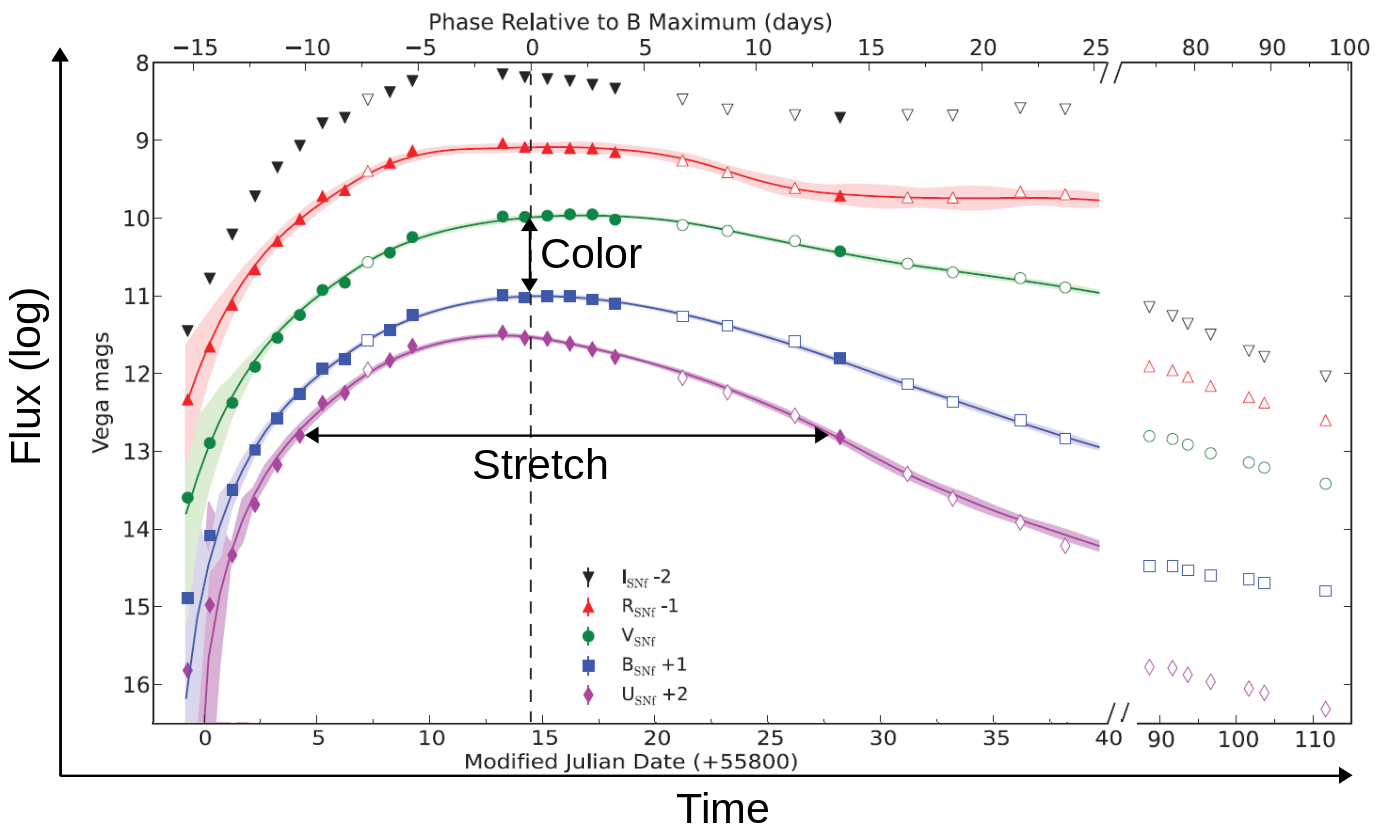
\includegraphics[width=.7\linewidth]{Rapport_figures/lightcurve.png}
    \captionsetup{justification=centering}
    \caption{Exemple de courbe de lumière d'une supernova depuis son explosion
    pour différentes longueurs d'ondes. On peut y définir un paramètre de
couleur et un paramètre de \textit{stretch} qui estime la durée d'explosion de
ladite SNe~Ia. \cite{pereira_spectrophotometric_2013}}
    \label{fig:lightcurves}
\end{figure}

Ainsi, la chandelle standard de la SNe~Ia est en réalité définie comme sa
luminosité dans la bande bleue ($\approx \SI{5000}{\A}$) à son maximum de
luminosité. \bigbreak

Les courbes de lumières des SNe~Ia sont paramétrées par trois éléments :

\begin{enumerate}
    \item Le maximum de luminosité dans la bande B, il s'agit du « $m$ des
        SNe~Ia » ;
    \item La couleur (« c »), définie par la différence de magnitude au maximum
        d'émission entre les bandes vertes et bleues ;
    \item Le \textit{stretch} (« $x_1$ »), définissant l'élargissement de la
        courbe de lumière.
\end{enumerate}

L'algorithme SALT2~\cite{guy_salt2_2007, guy_supernova_2010} permet d'ajuster
ces paramètres. La définition de ces paramètres n'est pas anodine : il existe
une corrélation entre $M_B$ (la magnitude absolue des SNe~Ia dérivée de $m_B$)
et le stretch $x_1$ et la couleur $c$ (mais pas entre $x_1$ et $c$ par
construction). Les SNe~Ia à évolution lente (grand stretch) ont une luminosité
intrinsèque plus grande (relation "brighter-slower")
\cite{phillips_absolute_1999} et les SNe~Ia les plus bleues sont plus lumineuses
(relation "brighter-bluer") \cite{tripp_two-parameter_1998, riess_first_2006}.
Ces relations sont illustrées figure \ref{brighter_slower_bluer}. \bigbreak

\begin{figure}[htbp!]
    \centering
    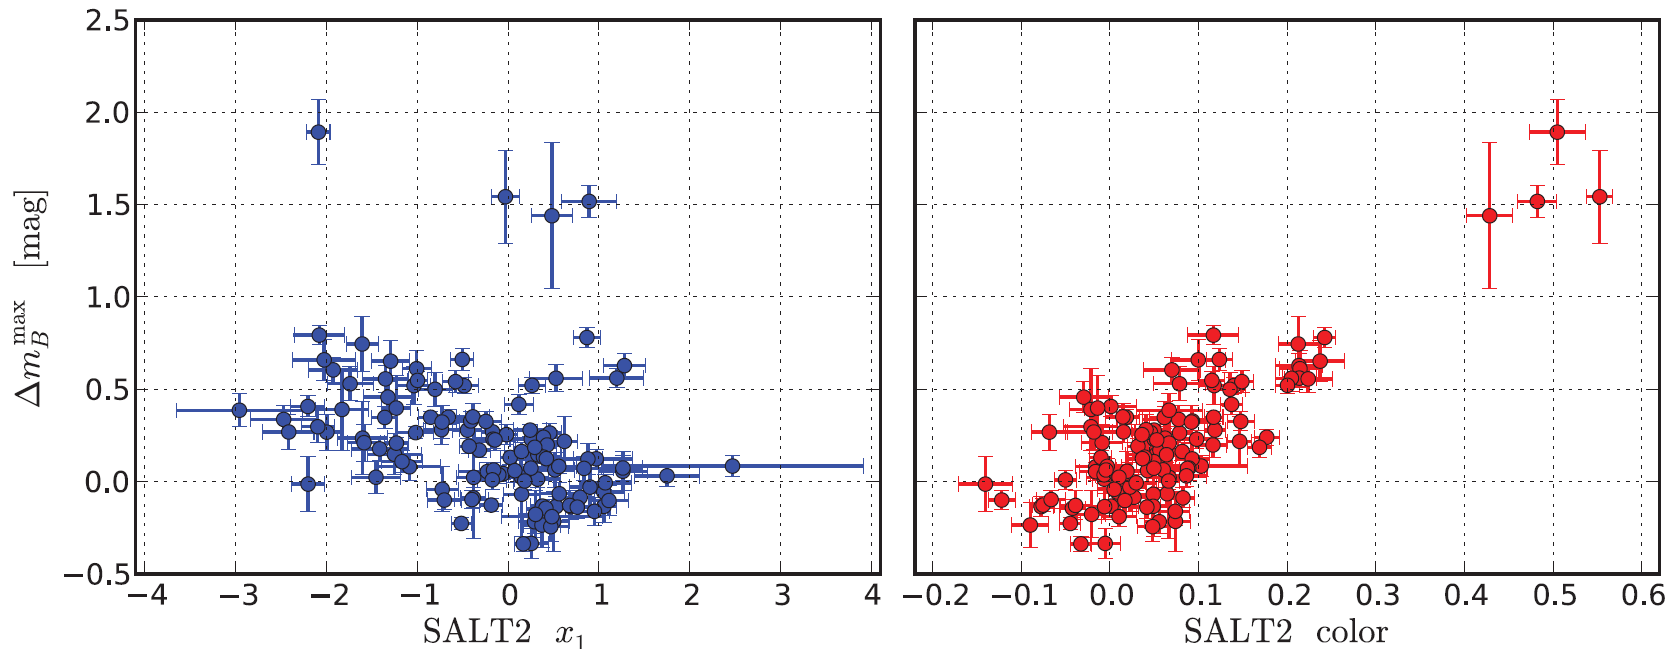
\includegraphics[width=.8\linewidth]{Rapport_figures/disp_x1_c.PNG}
    \captionsetup{justification=centering}
    \caption{Corrélations entre la différence de luminosité maximale d'une
    supernova dans le bleu et les paramètres de stretch (« $x_1$ ») et de
couleur (« color ») d'après l'algorithme SALT2.}
    \label{brighter_slower_bluer}
\end{figure}

Pour réduire la dispersion naturelle de magnitude absolue des SNe~Ia, on peut
alors inclure ces relations linéaires dans l'expression de la magnitude absolue,
de telle sorte que :

\begin{equation}
    M_B{}^{\text{corr}} \equiv M_B{}^{\text{max}} + \LF{\a x_1 - \b c}
\end{equation}

où $\a$ est le coefficient du stretch, et $\b$ celui de la couleur, tous les
deux positifs ; $M_B{}^{corr}$ est la nouvelle définition de la magnitude
absolue des SNe~Ia, dite « standardisée ». Ces trois paramètres sont ajustés
simultanément sur l'ensemble des données disponibles. \bigbreak

Ces relations supplémentaires permettent de réduire l'incertitude sur la
mesure de distance, puisque la dispersion de magnitude absolue est réduite à
$\approx 0.15 \mathrm{mag}$ \cite{betoule_improved_2014}, soit une précision en
distance de l'ordre de 8\%. La nouvelle définition du module de distance
(standardisé) des SNe~Ia est :

\begin{equation}
    \m = m - M +\a x_1 - \b c
\end{equation}

La réduction de la dispersion dans le diagramme de Hubble est illustrée figure
\ref{disp_20} avec les données de SNfactory \cite{rigault_strong_2018}.
\bigbreak

\begin{figure}[htbp!]
    \centering
    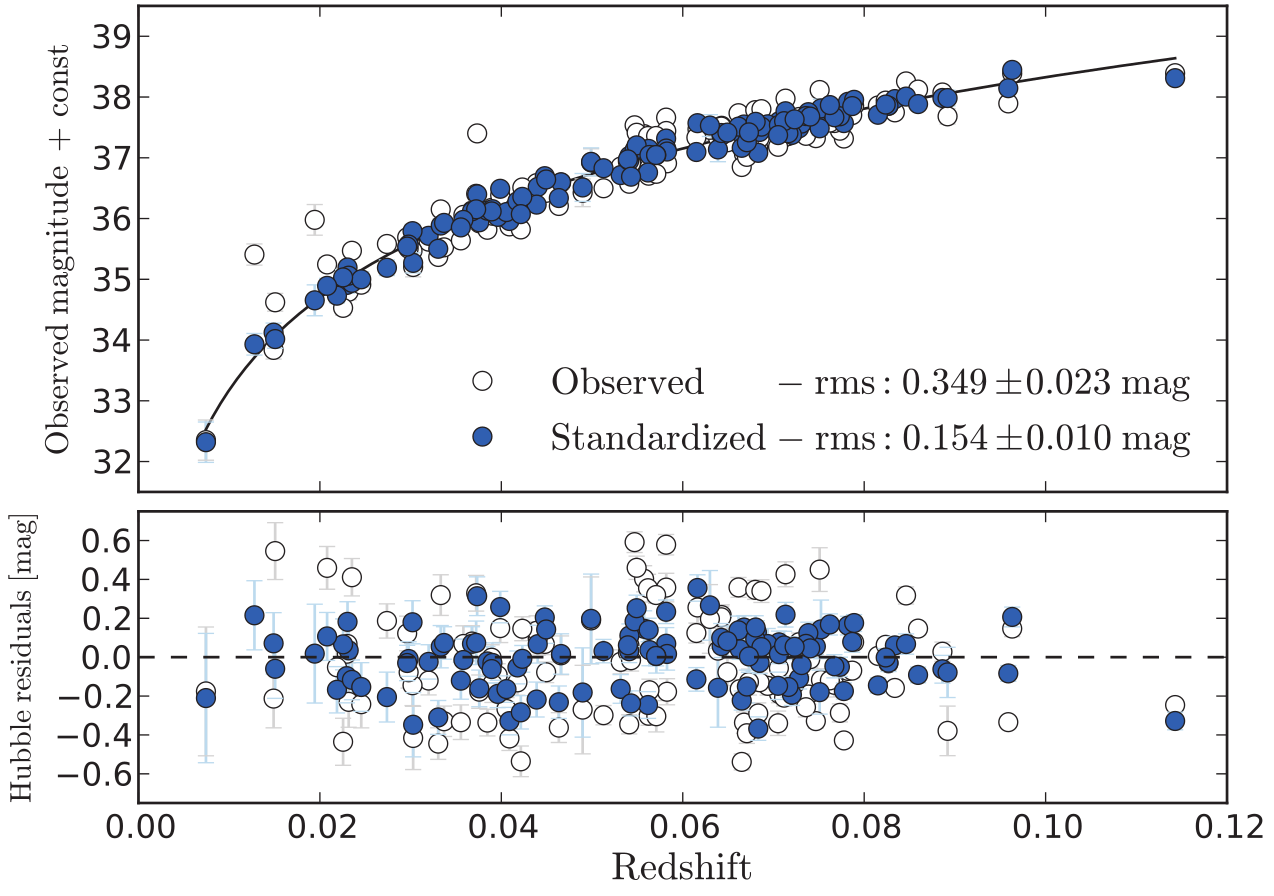
\includegraphics[width=.6\linewidth]{Rapport_figures/disp_beau.png}
    \captionsetup{justification=centering}
    \caption{Diagramme de Hubble avec, en haut, la magnitude apparente avant et
        après le processus de standardisation, qui consiste à inclure les
        corrélations entre la magnitude absolue et les paramètres de stretch et
        de couleur, respectivement en blanc et en bleu. En bas, on a le
        \textit{résidu} ne montrant que la dispersion autour de la courbe noire,
        indiquant l'évolution de la luminosité prédite par la loi de Hubble.}
    \label{disp_20}
\end{figure}

L'utilisation de cette relation a alors permis d'améliorer la précision des
mesures de distance, et ainsi discriminer différentes valeurs possibles pour les
paramètres cosmologiques : cela a mené à la découverte de l'expansion accélérée
de l'Univers \textit{via} une valeur non-nulle de $\O_\L$ pour laquelle un prix
Nobel a été decerné en 2011. La dernière compilation des SNe~Ia est
présentée fig~\ref{fig:hub_current}.

\begin{figure}[htbp!]
    \centering
    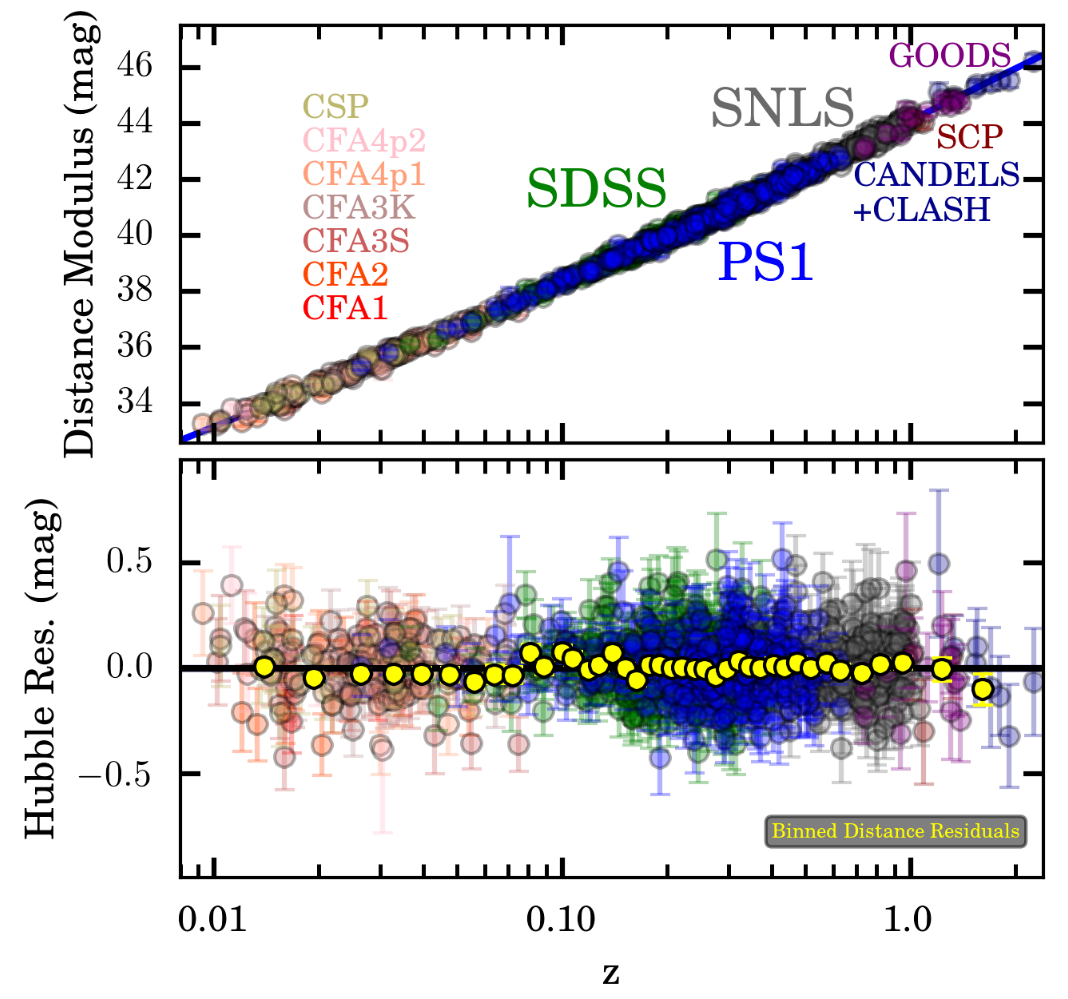
\includegraphics[width=.6\linewidth]{Rapport_figures/hub_current.png}
    \captionsetup{justification=centering}
    \caption{En haut, diagramme de Hubble actuel (en couleurs, une par
             échantillon d'observation) et diagramme résiduel où l'on a retiré
             l'évolution théorique du module de distance.
             \cite{scolnic_complete_2018}}
    \label{fig:hub_current}
\end{figure}

\subsection{Incertitudes systématiques}\label{ssec:syst}

Depuis la découverte de l'accélération de l'expansion de l'univers, qui ne se
basait que sur une centaine de données de SNe Ia, plus de données ont été
accumulées, et la précision sur les mesures de $\O_M$ et $\O_\L$ s'est
améliorée. Nous pouvons maintenant mesurer le paramètre d'équation d'état de
l'énergie noire $w$, qui devrait valoir $-1$ s'il s'agit d'une constante
cosmologique $\Lambda$. Aujourd'hui avec $\approx1000$ SNe~Ia, $w$ est mesuré
avec une précision de 5\% et est compatible avec -1 \cite{betoule_improved_2014,
scolnic_complete_2018}. Dans un futur proche (2022), le \textit{Large Synaptic
Survey Telescope} (LSST, récemment renommé \textit{Vera Rubin Survey Telescope})
installé au Chili devrait acquérir $\approx 10000$ SNe~Ia par an. Un des
objectifs principaux du sondage cosmologique est de mesurer $w$ au pourcent,
mais surtout, de mesurer $w_a$, l'évolution potentielle de $w$ en fonction du
temps, à 10\% ; $w_a$ devrait être 0 si l'énergie noire est une simple constante
cosmologique.  Cependant, déjà aujourd'hui, les erreurs systématiques dominent
le budget total d'erreur de la mesure des paramètres cosmologiques avec les
SNe~Ia, comme illustré fig~\ref{fig:scolnic_syst}. \bigbreak

\begin{figure}[htbp!]
    \centering
    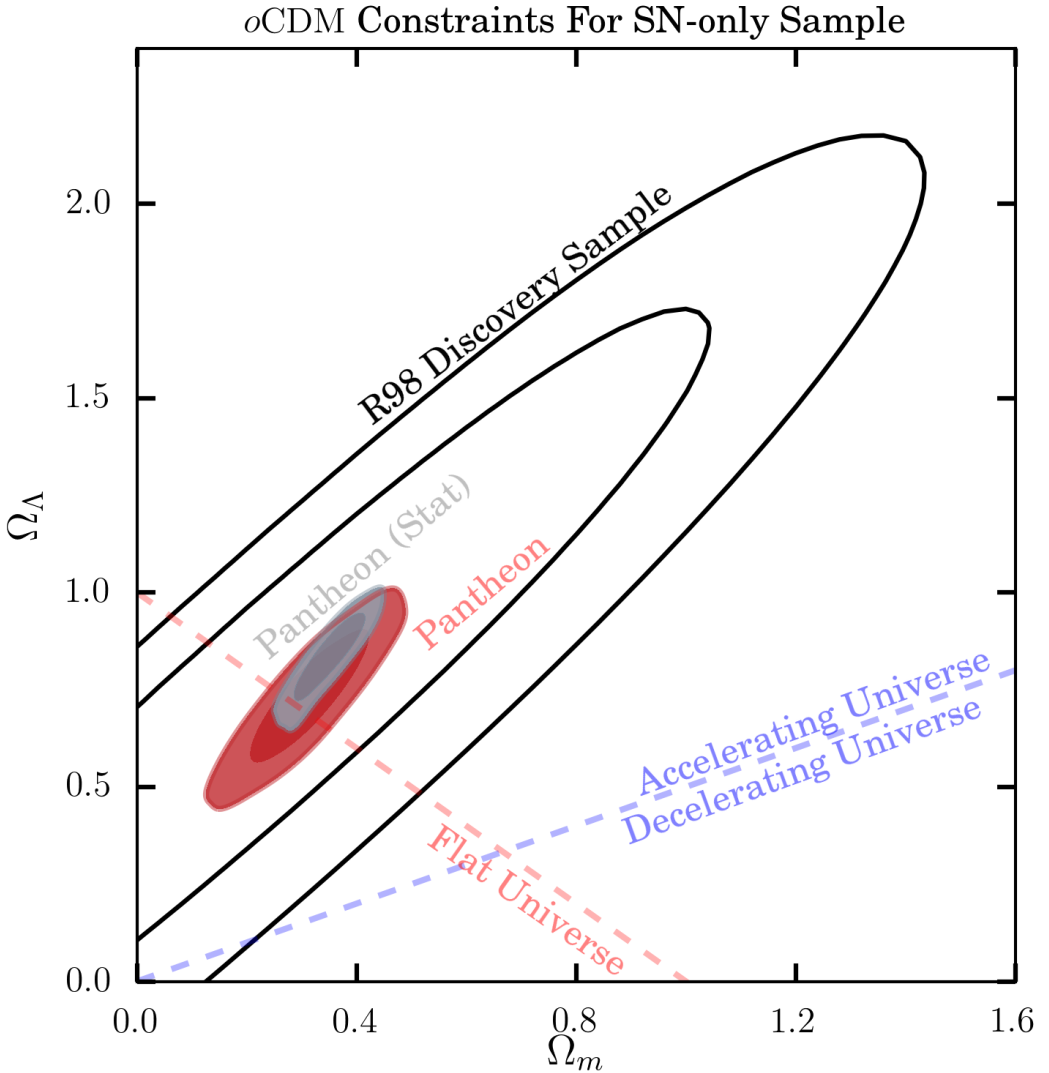
\includegraphics[width=.5\linewidth]{Rapport_figures/scolnic_syst.png}
    \captionsetup{justification=centering}
    \caption{\textit{Contour plot} indiquant la précision à 68 et 90\% de la
    mesure des paramètres $\O_M$ et $\O_\L$ pour la découverte historique de
    \bsc{Riess et. al} (R98, en blanc) se basant sur 100 données de SNe Ia, et
    pour les échantillons actuels utilisant environ 1000 SNe Ia (en rouge). En
    gris est indiquée la part des incertitudes statistiques à l'incertitude
    totale. \cite{scolnic_complete_2018}}
    \label{fig:scolnic_syst}
\end{figure}

\begin{figure}[htbp!]
    \centering
    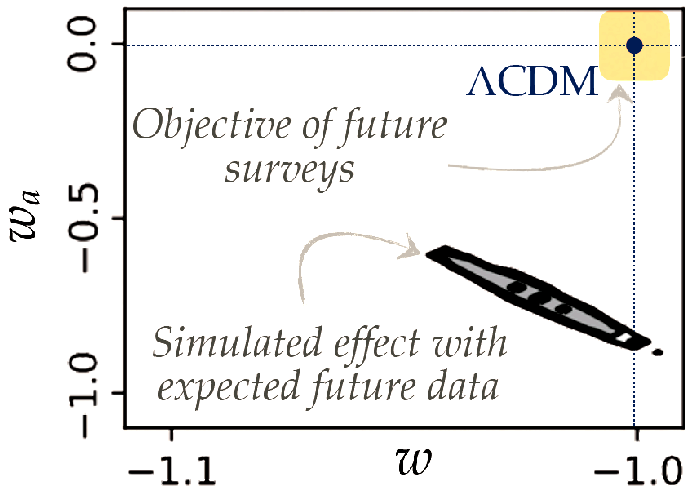
\includegraphics[width=.5\linewidth]{Rapport_figures/error.pdf}
    \captionsetup{justification=centering}
    \caption{Erreur attendue sur la mesure de $w$ et $w_a$ en ne considérant
    que la réduction des erreurs statistiques sans prendre en compte les erreurs
    systématiques.}
    \label{fig:err_syst}
\end{figure}

Pour continuer à améliorer les mesures cosmologiques, il est donc nécessaire de
travailler sur les sources d'erreurs systématiques, faute de quoi il sera
impossible d'exploiter l'immense masse de données fournie par LSST. Une des
erreurs dominantes et encore peu étudiée est l'impact de notre connaissance
limitée de la physique des SNe~Ia sur la mesure des paramètres cosmologiques
\cite{rigault_strong_2018} et notamment sur l'évolution potentielle de
$M_B^{\mathrm{corr}}$ en fonction du redshift. La fig~\ref{fig:err_syst} montre
une estimation de l'impact potentiel qu'aurait une évolution réaliste de la
physique des SNe~Ia en fonction du temps sur l'estimation des paramètres ($w$,
$w_a$).  Non seulement l'erreur systématique associée est plus grande que la
précision souhaitée pour LSST, mais surtout la zone mesurée est en désaccord
complet avec ce qui est attendu. La mesure est donc non seulement moins précise,
mais elle est aussi faussée. C'est dans ce cadre que s'inscrit mon stage et la
thèse qui en découle.

\section{Construction de l'échantillon d'étude}\label{sec:complet}

Dans ce stage, nous avons cherché à mesurer si la propriété intrinsèque de
stretch des SNe~Ia changeait en fonction du temps, ou, ce qui est équivalent, du
redshift. Comme nous l'avons vu section~\ref{ssec:lc}, le stretch est une
propriété purement intrinsèque à l'explosion du progéniteur en SNe~Ia. Ainsi, si
nous pouvons détecter une évolution de la distribution de stretch en fonction du
redshift, alors nous aurons prouvé qu'en effet les SNe~Ia changent avec le
temps. Il nous faut donc comparer des SNe~Ia dans plusieurs gammes de redshift
et comparer leurs distributions de stretch. Cependant, les effets de sélection
affectent ces distributions : il est donc dans un premier temps
nécessaire de savoir quelles SNe~Ia sont affectées ou non par ces effets de
sélection. \bigbreak

Nous discutons les effets de sélection plus en détails
section~\ref{ssec:selec}, puis, dans la section~\ref{ssec:det} nous montrons
comment construire un échantillon complet (i.e. affranchis des effets de
sélection) ; échantillons que nous utiliserons par la suite pour nos analyses
(cf. section~\ref{sec:stretchevol}).

\subsection{Effets de sélection}\label{ssec:selec}

L'observation du nombre de SNe Ia en fonction du redshift illustre l'existence
d'effets de sélection : si l'on suppose une répartition homogène et isotrope des
supernovae dans l'espace, alors on s'attend à avoir un nombre croissant de
SNe~Ia avec le redshift ($z$), tel que $N_{\text{SNe~Ia}} \propto z³$. Mais
lorsque l'on regarde la distribution de SNe~Ia en fonction du redshift, comme
montré fig~\ref{fig:redshift_miss} pour l'échantillon de SNLS
\cite{astier_supernova_2006, betoule_improved_2014}, si cette relation semble
vérifiée jusqu'à une certaine distance (la distribution croît), nous constatons
qu'à partir d'un certain redshift, le nombre de SNe~Ia observé réduit. Dans ce
cas, la transition semble s'effectuer autour de $z\approx0.7$. \bigbreak

\begin{figure}[htbp!]
    \centering
    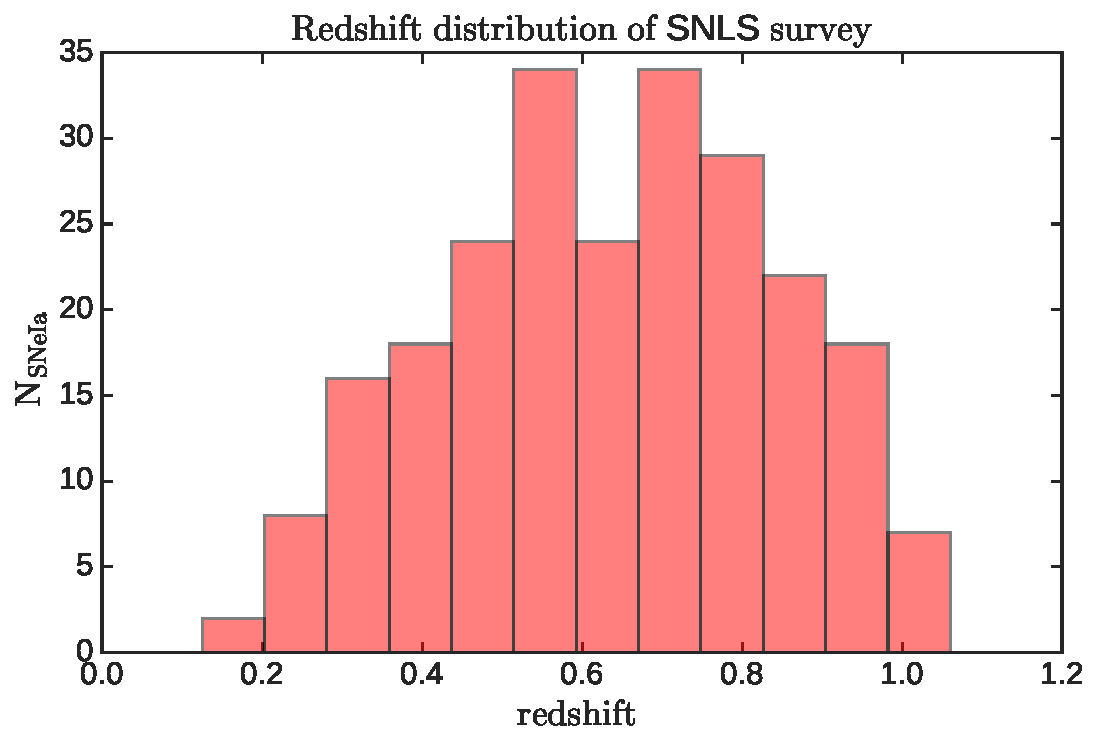
\includegraphics[width=.6\linewidth]{Rapport_figures/dist_SNLS.pdf}
    \captionsetup{justification=centering}
    \caption{Histogramme du nombre de SNe Ia observées en fonction du redshift
    pour les données de l'échantillon SNLS (SuperNova Legacy Survey).}
    \label{fig:redshift_miss}
\end{figure}

Pour comprendre cette distribution, rappelons nous que nous mesurons l'évolution
du flux des SNe~Ia pour en dériver la distance (voir section~\ref{ssec:hub}).
Or, les instruments (caméras ou spectrographes) ont une limite de détection de
flux en-dessous de laquelle les objets ont une luminosité trop faible pour être
détectée. Pour les SNe~Ia, qui ont toutes une luminosité relativement similaire, cela signifie qu'à partir d'une certaine distance, leur flux sera trop faible
pour être détecté. C'est ce que nous observons fig.~\ref{fig:redshift_miss} : à
$z\lesssim0.7$ toutes les SNe~Ia sont assez lumineuses pour etre observées, à
$z\gtrsim 0.7$ les SNe~Ia relativement sous-lumineuses manquent en premier, puis
celles de moins en moins lumineuses jusqu'à ce qu'elles soient toutes trop
faibles car trop lointaines. \bigbreak

Si cette sélection en luminosité était indépendante du stretch alors il n'y
aurait pas de problème, nous pourrions utiliser toutes les SNe~Ia pour notre
analyse. Cependant, comme discuté section~\ref{ssec:lc}, à cause de la relation
"brighter-slower", les SNe~Ia les moins lumineuses sont également celles qui ont
un plus petit stretch en moyenne. Ainsi, une fois passé un certain redshift (ici
$z\sim0.7$) la distribution de stretch de l'échantillon n'est plus
représentative de ce que la nature fournit. C'est pourquoi, pour étudier
l'évolution de la distribution de stretch des SNe~Ia en fonction du redshift, il
faut exclure les SNe~Ia au-delà de ce redshift caractéristique qui dépend de
l'instrument utilisé, et donc de l'échantillon. \bigbreak

L'objectif est donc de trouver, pour chaque échantillon, la valeur de ce
redshift caractéristique et de considérer seulement les SNe~Ia de cet
échantillon disposant d'un redshift inférieur à ce redshift limite. Nous pouvons
ensuite combiner les SNe~Ia des différents échantillons pour notre étude du
stretch en fonction du redshift puisqu'elles seront toutes représentatives de ce
que la nature crée.

\subsection{Détermination du redshift limite}\label{ssec:det}

Pour déterminer le redshift limite au delà duquel les effets de sélection
deviennent non-négligeables, l'approche qui a été choisie repose sur la
comparaison entre l'évolution attendue du nombre de SNe~Ia par intervalle de
redshift et l'évolution observée. Une étude plus rigoureuse aurait été de
s'intéresser aux caractéristiques de limite de détection de chaque instrument,
mais nous ne disposions pas, pour ce stage, de ces informations. \bigbreak

Comme discuté précédemment, on s'attend à avoir un nombre de supernovae qui
croît proportionnellement à $z³$. En utilisant l'histogramme précédent, on a,
pour chaque intervalle, le nombre de supernovae observées. En définissant une
fonction de paramètre $a$ telle que $N_{\text{SNe~Ia}} = a\times V(z)$, où
$V(z)$ est le volume d'univers à un redshift donné, on peut trouver pour chaque
milieu d'intervalle le nombre attendu de supernovae observées selon cette
fonction. On peut alors utiliser une statistique poissonienne pour trouver la
probabilité d'avoir ce nombre attendu sachant qu'on en a effectivement observé
le nombre correspondant aux intervalles. Le paramètre libre $a$ est dérivé
en maximisant cette probabilité. \bigbreak

Comme illustré figure \ref{fig:zmax_method}, lorsqu'on dérive $a$ en ne
considérant que les premiers intervalles de redshift la correspondance est
bonne. On augmente ensuite le redshift limite utilisé pour dériver $a$ et on
compare la qualité de la minimisation. Le redshift limite est celui à partir
duquel la qualité de la minimisation décroît. Cependant, cette méthode dépend du
choix initial du nombre d'intervalles de redshift. Pour s'affranchir de cela
nous avons, pour chaque échantillon, appliqué 100 fois la méthode précédente en
changeant à chaque fois de manière aléatoire le nombre d'intervalles (entre 5 et
13) tout en changeant les bornes globales de redshift inférieure et supérieure.
\bigbreak

\begin{figure}[htbp!]
    \centering
    \subfigure[7
    premiers]{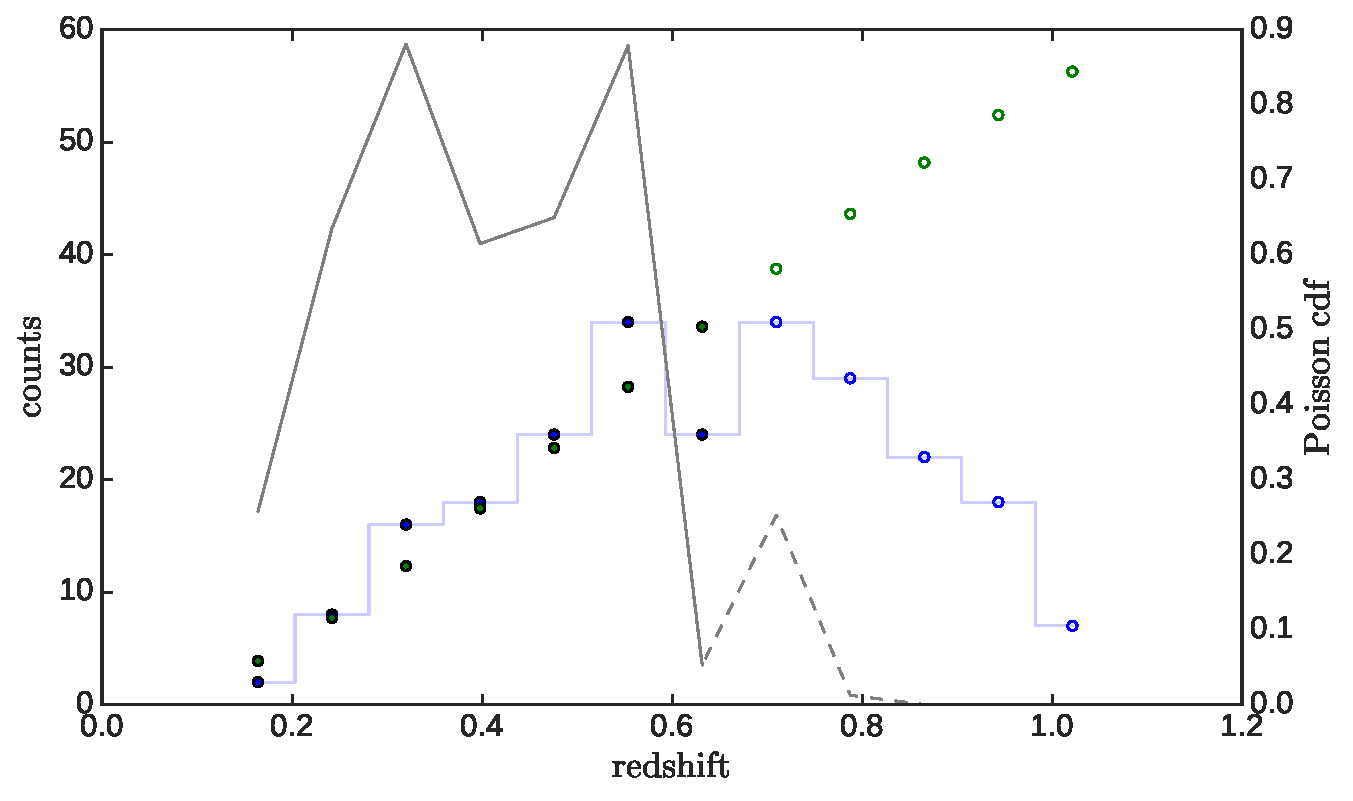
\includegraphics[width=.45\textwidth]{Rapport_figures/zmax_method_7.pdf}}
    \subfigure[9
    premiers]{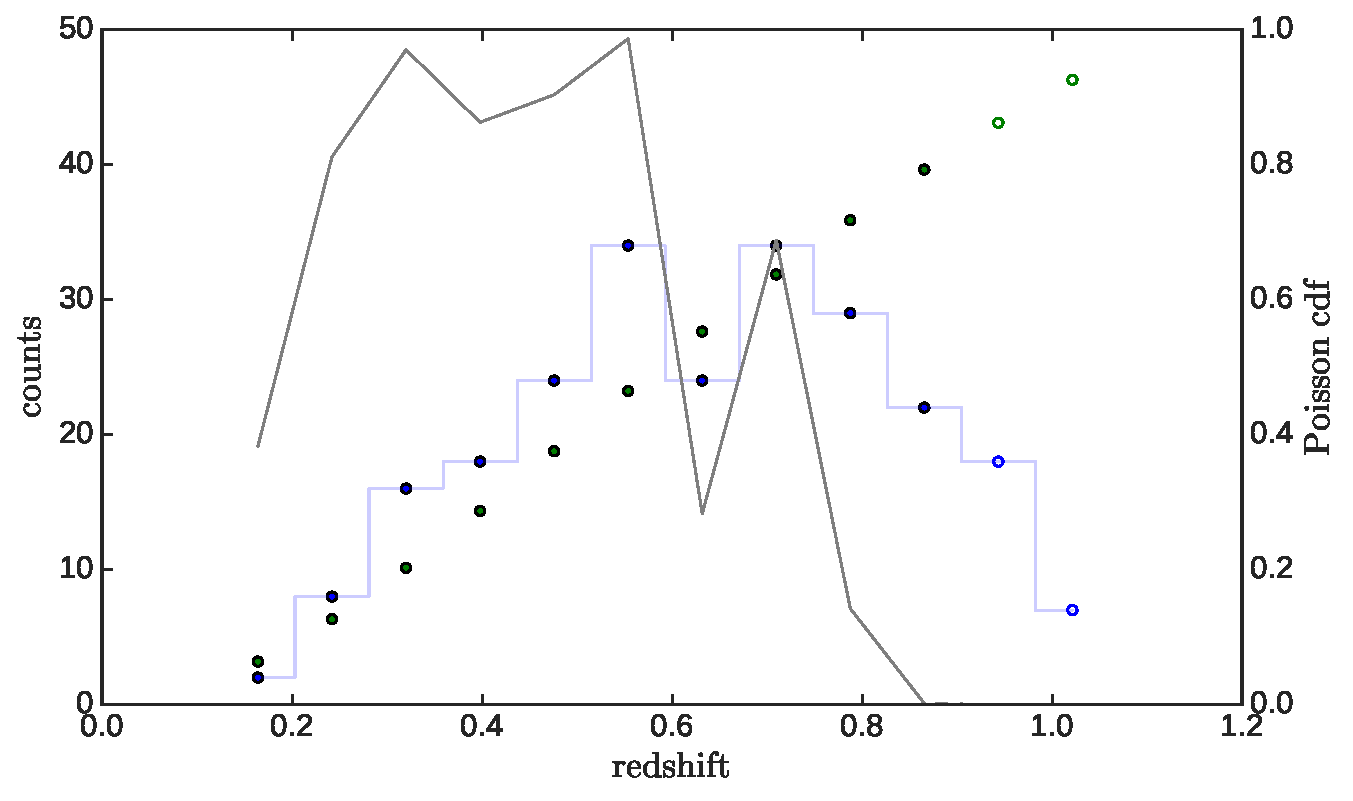
\includegraphics[width=.45\textwidth]{Rapport_figures/zmax_method_9.pdf}}
    \captionsetup{justification=centering}
    \caption{Graphique présentant l'évolution de la probabilité poissonienne
        d'observer un nombre de supernovae correspondant à la fonction
        $N_{\text{SNe~Ia}} = a\times V(z)$ sachant que l'on en a observé le
        nombre correspondant à l'intervalle. En pointillés est représenté ce
        que l'on obtiendrait en extrapolant ce que cette probabilité deviendrait
        en prenant plus d'intervalles.}
    \label{fig:zmax_method}
\end{figure}

Les courbes d'évolution de la probabilité poissonienne sont enregistrées puis
interpolées linéairement. La figure~\ref{fig:zmax_result} montre l'évolution
médiane (et écart-type pour la bande d'erreur) de la probabilité que le nombre
de SNe~Ia observées par l'échantillon considéré à un redshift donné soit
compatible avec celui attendu si l'échantillon était complet. Le redshift
maximal est celui à partir duquel on est à 30\% de cette probabilité. Les
conséquences du choix de cette valeur sur les résultats de l'analyse qui en
découle seront testées par la suite.

\begin{figure}[htbp!]
    \centering
    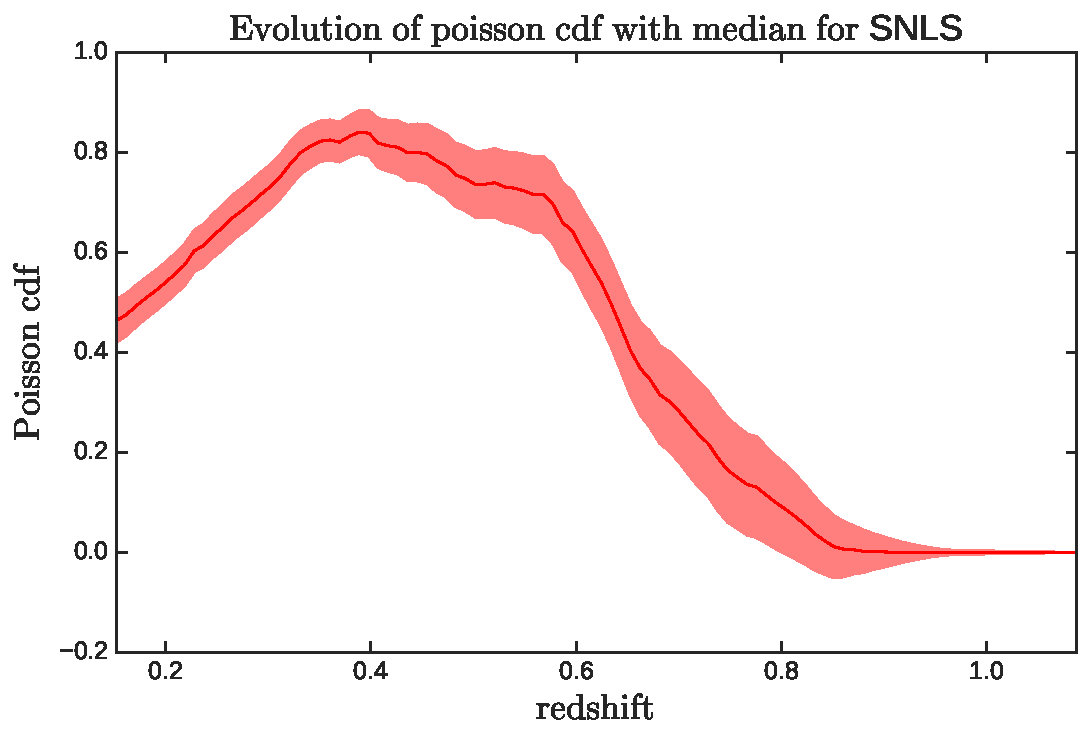
\includegraphics[width=.6\linewidth]{Rapport_figures/zmax_SNLS.pdf}
    \captionsetup{justification=centering}
    \caption{Résultat du procédé de détermination du redshift maximal à partir
    duquel les effets de sélections ne sont pas anodins.}
    \label{fig:zmax_result}
\end{figure}

\subsection{Échantillon utilisé}

Une fois déterminé le redshift limite pour chacune des sources de SNe~Ia, nous
pouvons constituer notre échantillon d'étude. Celui-ci est, par construction,
représentatif de ce que la nature produit. La table~\ref{tab:sample} récapitule
l'origine des SNe~Ia et la fig.~\ref{fig:surveys_cuts} montre le stretch en
fonction du redshift pour toutes les SNe~Ia considérées (sauf SNfactory et HST,
voir ci-après) ; celles que nous utiliserons ont un marqueur plein.  \bigbreak

\begin{table}[htbp!]
    \centering
    \captionsetup{justification=centering}
    \caption{Nombre de SNe~Ia pour chaque échantillon complet}
    \label{tab:sample}
    \begin{tabularx}{\linewidth}{|Y*{1}{|Y}|}\hline
        \rowcolor{gray!15} Échantillon & Nombre de SNe~Ia \\\hline\hline
        SNf & 141 \\\hline
        PS1 & 178 \\\hline
        SDSS & 206 \\\hline
        SNLS & 138 \\\hline
        HST & 26 \\\hline
    \end{tabularx}
\end{table}

\begin{figure}[htbp!]
    \centering
    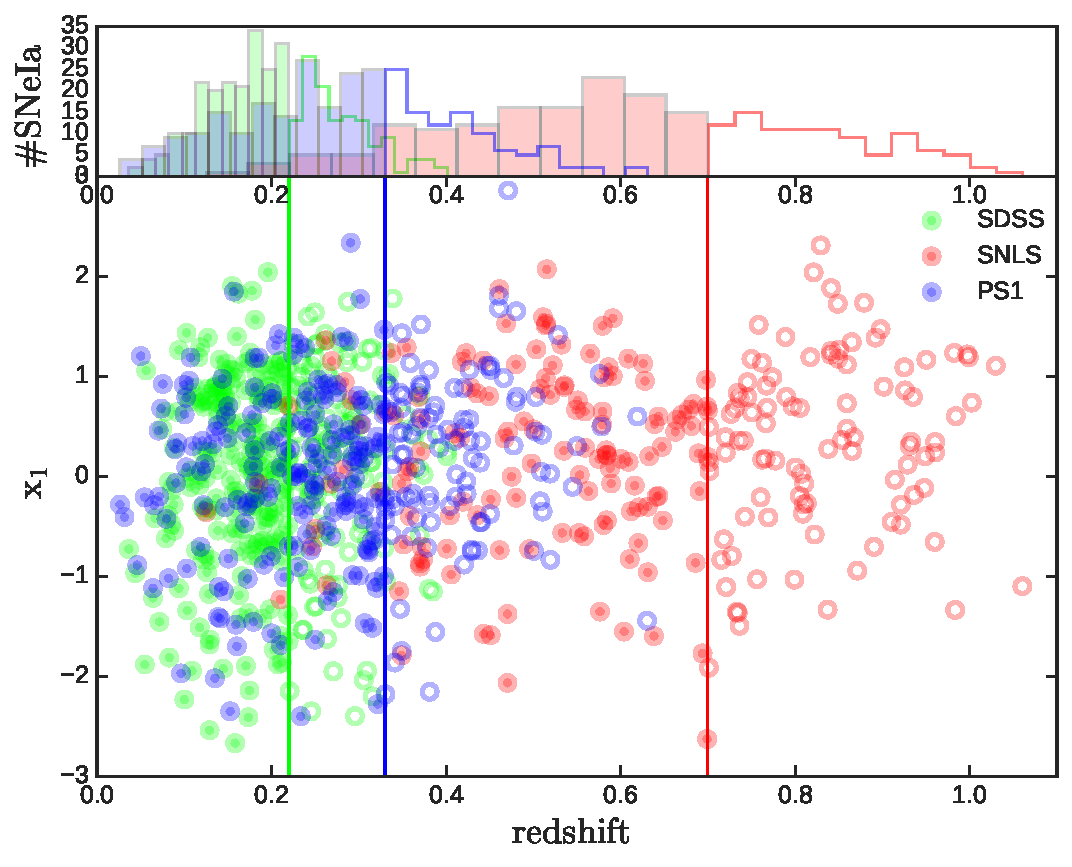
\includegraphics[width=.7\linewidth]{Rapport_figures/surveys_cuts.pdf}
    \captionsetup{justification=centering}
    \caption{Représentation des données des échantillons subissant des effets
    de sélection après application du procédé : les points creux représentent
    les données ignorées.}
    \label{fig:surveys_cuts}
\end{figure}

Aux trois échantillons provenant de \cite{scolnic_complete_2018} et dont nous
avons extrait notre échantillon complet, peut s'ajouter un quatrième
échantillon, celui de the Nearby Supernova factory (SNfactory)
\cite{wood-vasey_nearby_2004} et les données proviennent de
\cite{rigault_strong_2018}.  Contrairement aux autres sondages, SNfactory
utilise des sondages indépendants pour trouver les SNe~Ia qu'il suit. Ces
derniers ont un niveau de détection plus profond que les autres et ainsi,
l'échantillon de SNfactory n'est pas affecté par des effets de sélection
\cite{rigault_strong_2018}. Nous utiliserons donc l'ensemble des données
provenant de ce sondage (voir~\ref{tab:sample}). Il en va de même pour les
quelques SNe~Ia à grand redshift mesurées par le Hubble Space Telescope (HST)
issues de \cite{scolnic_complete_2018}. \bigbreak

Notre échantillon est donc constitué de 689 SNe~Ia couvrant un domaine de
redshift allant de $z=0.02$ à $z=2.26$.

\section{Évolution intrinsèque des SNe~Ia}\label{sec:stretchevol}

En plus des données liées aux courbes de lumière (stretch, couleur, magnitude),
les données de SNfactory disposent également d'une mesure de la probabilité
qu'une SNe~Ia soit issue d'un progéniteur jeune ($\lesssim \SI{500}{Myr}$) ou
vieux ($\gtrsim \SI{1}{Gyr}$). \cite{rigault_strong_2018} ont montré une
corrélation forte entre le stretch des SNe~Ia et le \textit{Local specific star
formation rate} (LsSFR), le traceur de la probabilité qu'une SNe~Ia soit jeune
ou vieille. Cette corrélation est montrée fig~\ref{fig:snf_data}.

\begin{figure}[htbp!]
    \centering
    \subfigure[Données brutes]{\label{fig:snf_data}
        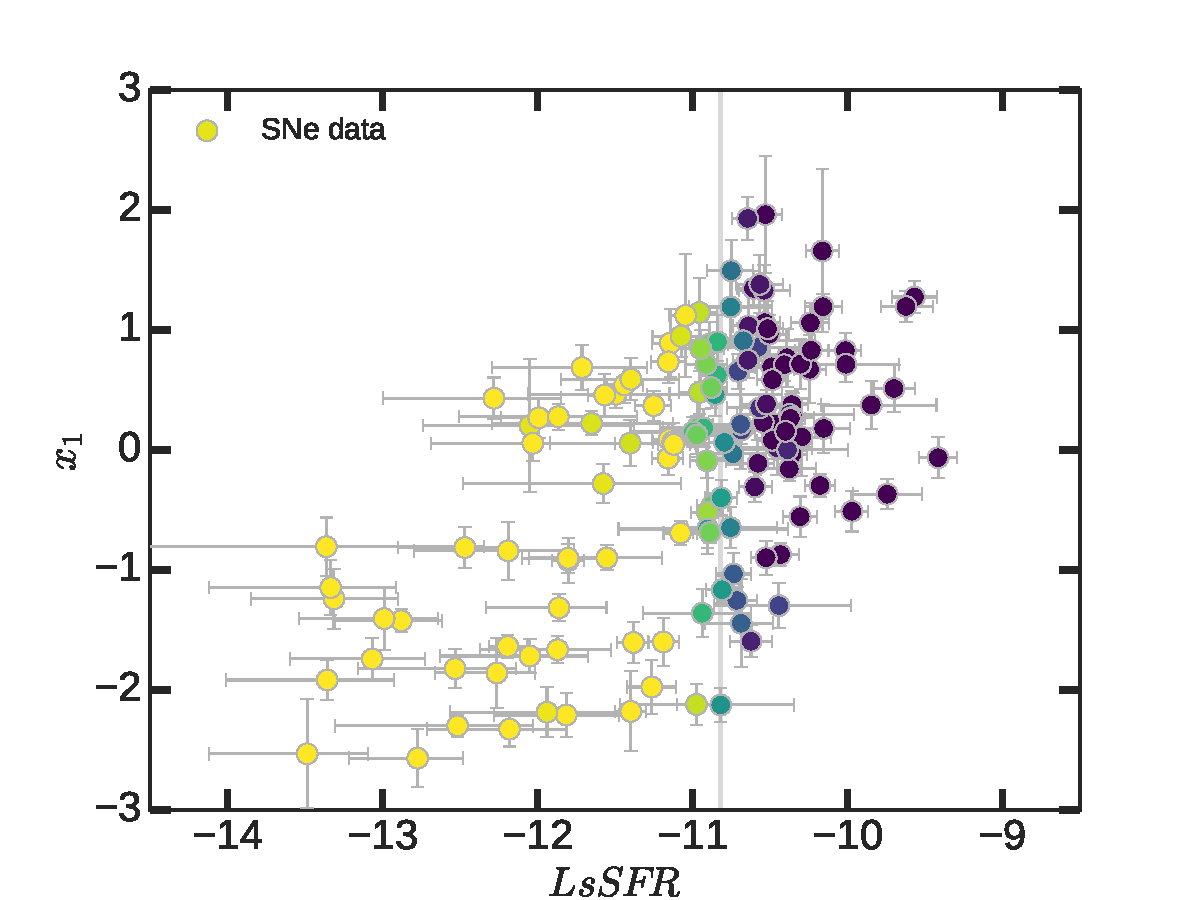
\includegraphics[width=.45\linewidth]{Rapport_figures/BiGaussian_onlydata.pdf}}
        \subfigure[Premier modèle mis en place]{\label{fig:3G2M2SSNF}
        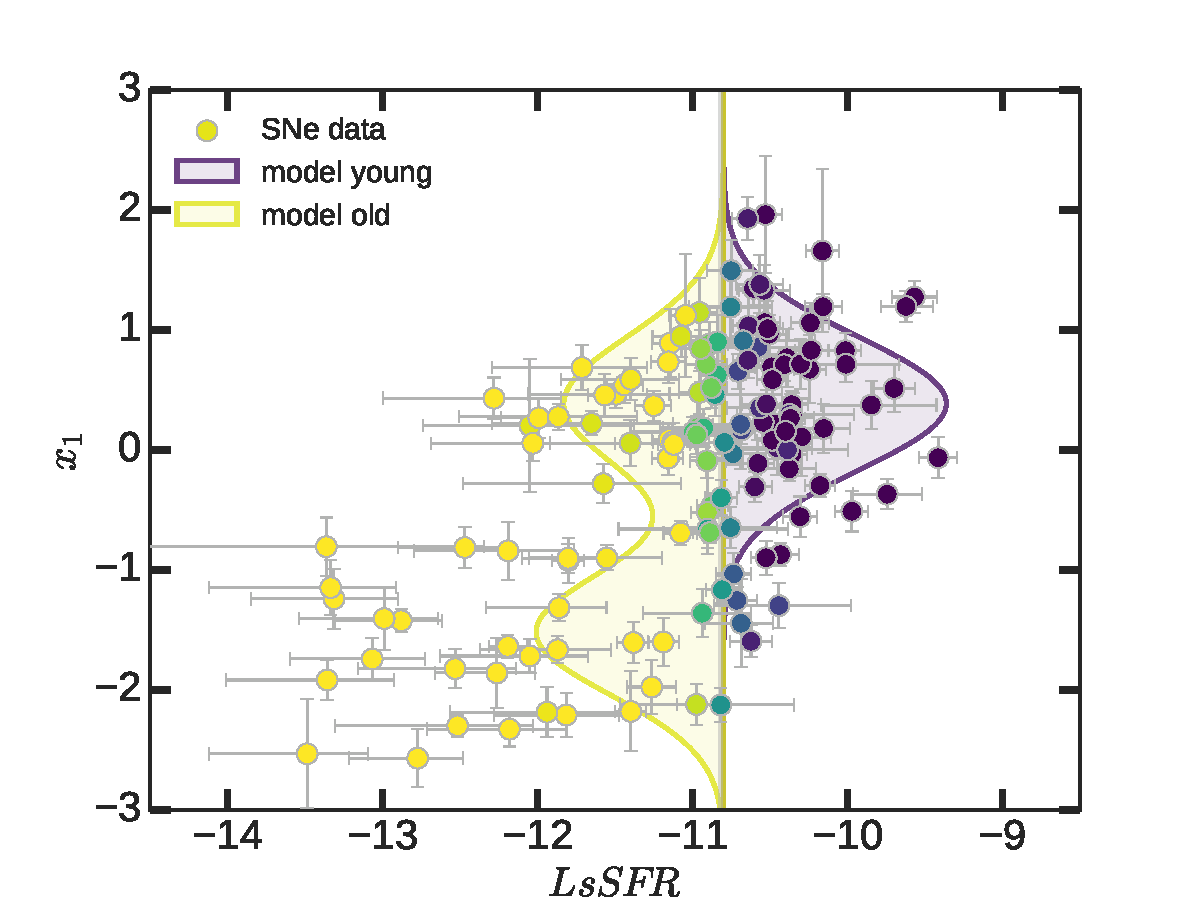
\includegraphics[width=.45\linewidth]{Rapport_figures/BiGaussian.pdf}}
    \captionsetup{justification=centering}
    \caption{Stretch des supernovae étudiées par la collaboration SNF en
    fonction de log(LsSFR). La couleur représente la probabilité pour une
supernova d'être issue d'un jeune progéniteur.}
\end{figure}

Le LsSFR est le ratio entre le taux de formation stellaire (SFR, traceur du
nombre de jeunes étoiles) et la masse (traceur du nombre d'étoiles largement
dominé par celles de la séquence principale comme le soleil). Or, le taux de
formation d'étoiles dans l'univers est très dépendant du redshift et est maximum
vers un redshift de 2, quand l'univers avait approximativement le tiers de son
âge actuel \cite{madau_cosmic_2014}. Il y avait ainsi $\approx40$ fois plus de
formation d'étoiles à un redshift de 1 qu'aujourd'hui. La masse n'évolue que
lentement avec le redshift. Puisque le stretch et le LsSFR sont corrélés, il est
donc probable que la distribution de stretch des SNe~Ia évolue également avec le
redshift. \bigbreak

Pour tester cette hypothèse, nous allons dans un premier temps construire un
modèle décrivant la distribution de stretch en fonction du LsSFR. Ce modèle est
présenté section~\ref{ssec:stretchevol_ori} où nous présentons également le
modèle d'évolution du LsSFR en fonction du redshift donné dans
\cite{rigault_strong_2018}. Dans la section~\ref{ssec:model} nous testerons ce
modèle sur les données de la littérature. Nous généraliserons ensuite ce modèle
dans la section~\ref{ssec:comp} et nous comparerons différents modèles, y
compris des modèles sans évolution avec le redshift, afin de déterminer lequel
est le plus probable.

\subsection{Modèle SNf d'évolution du stretch}\label{ssec:stretchevol_ori}

\cite{rigault_strong_2018} appellent $\de\z$ la fraction de jeunes étoiles dans
un échantillon et $\psi\z$ la fraction de vieilles. Suivant
\cite{mannucci_supernova_2005, scannapieco_type_2005, sullivan_rates_2006}, ils
supposent que les fractions de jeunes et vieilles étoiles sont respectivement
proportionnelles au SFR et à la masse stellaire. Le ratio des deux est donc
proportionnel au LsSFR qui évolue comme $(1+z)^{2.8\pm0.2}$ d'après
\cite{tasca_evolving_2015}. Ainsi \cite{rigault_strong_2018} donne :

\begin{equation}
\label{eq:lssfr}
    \frac{\de\z}{\psi\z} \equiv LsSFR\z = K\times \LF{1+z}^{\f}
\end{equation}
avec $\f=2.8$. Sachant que $\de\z + \psi\z = 1$, on a:
\begin{align}
\label{eq:depsi}
    \de\z &= \LF{K⁻¹\times \LF{1+z}^{-\f} + 1}⁻¹\ ;\\
    \psi\z &= \LF{K\times \LF{1+z}^{+\f} + 1}⁻¹
\end{align}

La valeur de LsSFR séparant les jeunes et vieilles SNe~Ia est choisie telle
qu'il y ait autant de supernovae de chaque sorte dans l'échantillon de
SNfactory, à $z\approx0.05$, ce qui impose $K=0.87$. \bigbreak

En s'appuyant sur la forme du nuage de point montré fig.~\ref{fig:snf_data},
notre modèle de distribution du stretch pour les jeunes et les vieilles SNe~Ia a
été le suivant :

\begin{itemize}
    \item \textbf{jeunes} : une gaussienne de moyenne $\m_1$ et d'écart type
        $\s_1$, soit $\mathcal{N}_1\equiv\mathcal{N}(\m_1, \s_1)$, 
    \item \textbf{vieilles} : une combinaison linéaire entre $\mathcal{N}_1$
        (même que pour les jeunes) et une seconde gaussienne
        $\mathcal{N}_2\equiv\mathcal{N}(\m_2, \s_2)$.
\end{itemize}

Ainsi, la probabilité d'observer une SNe~Ia "i" jeune avec un stretch $x_1^i$
d'erreur $\d x_1^i$ est:

\begin{equation}
    p(x_1^i, \d x_1^i | \m_1, \s_1) = \mathcal{N}\left(\m_1,
    \sqrt{\s_1{}^2+\d x_1^i{}^{2}}\right)(x_1^i)
\end{equation}
et pour une SNe~Ia vieille :
\begin{align}
    \label{eq:prob}
    p(x_1^i, \d x_1^i | \m_{1,2}, \s_{1,2}, a) = a & \times \mathcal{N}
    \LF{\m_1, \sqrt{\s_1{}^2 + \d x_1^i{}^{2}}} (x_1^i) \ + \\
    (1-a) & \times \mathcal{N} \LF{\m_2, \sqrt{ \s_2{}^2 + \d x_1^i{}^{2}}}
    (x_1^i), \nonumber
\end{align}

\noindent où $a$ est le facteur d'amplitude relative entre les deux modes
$\mathcal{N}_1$ et $\mathcal{N}_2$. En ajustant ce modèle sur les données de
SNfactory (voir fig.~\ref{fig:snf_data}), nous trouvons les résultats table
\ref{tab:val}.  Pour une question de nomenclature pour la suite, nous
désignerons ce modèle : 3G2M2S$_{\mathrm{SNf}}$, car il est composé de 3
gaussiennes (deux vieilles, une jeune) mais composé de seulement deux valeurs
centrales $\m$ et deux écart-types $\s$ et dont tous les paramètres libres ont
été ajustés sur les données de SNf.

\begin{table}[htbp!]
    \centering
    \captionsetup{justification=centering}
    \caption{Valeurs des paramètres pour différents modèles. En rouge les
    données aberrantes.}
    \label{tab:val}
    \begin{tabularx}{\linewidth}{|Y*{6}{|Y}|}\hline

        \rowcolor{gray!15} Modèle & $a$ & $f$ & $\m_1$ & $\s_1$ & $\m_2$ &
        $\s_2$ \\\hline\hline

        3G2M2S$_{\mathrm{SNf}}$ & $0.48 \pm 0.07$ & none & $0.39 \pm 0.07$ &
        $0.56 \pm 0.05$ & $-1.5 \pm 0.1$ & $0.52 \pm 0.09$ \\\hline

        3G2M2S & $0.48 \pm 0.17$ & none & $0.36 \pm 0.08$ & $0.61 \pm 0.05$ &
        $-1.3 \pm 0.2$ & $0.60 \pm 0.12$ \\\hline

        3G2M2SF & \textcolor{red}{$0.1 \pm 0.6$} & \textcolor{red}{$0.2 \pm
        0.6$} & $-0.9 \pm 0.7$ & $0.7 \pm 0.3$ & $0.5 \pm 0.2$ & $0.6 \pm 0.1$
        \\\hline

        3G2M1S & $0.47 \pm 0.07$ & none & $0.35 \pm 0.04$ & $0.61 \pm 0.03$ &
        $-1.25 \pm 0.10$ & $\s_1$ \\\hline

        3G2M1SF & \textcolor{red}{$0.2 \pm 0.9$} & $0.7 \pm 0.3$ & $0.36 \pm
        0.04$ & $0.60 \pm 0.03$ & $-1.23 \pm 0.10$ & $\s_1$ \\\hline

        2G2M2S & none & none & $0.49 \pm 0.04$ & $0.54 \pm 0.03$ & $-0.72 \pm
        0.08$ & $0.83 \pm 0.07$ \\\hline
        
        2G2M2SF & none & $0.3 \pm 0.2$ & $-0.9 \pm 0.6$ & $0.7 \pm 0.2$ & $0.5
        \pm 0.2$ & $0.56 \pm 0.09$ \\\hline

    \end{tabularx} \bigbreak

\begin{tabularx}{\linewidth}{|Y*{2}{|Y}|}\hline

    \rowcolor{gray!15} Modèle & $\m$ & $\s$ \\\hline\hline

    1G1M1S & \textcolor{red}{$0.01 \pm 0.04$} & $0.90 \pm 0.03$ \\\hline

\end{tabularx} \bigbreak

\begin{tabularx}{\linewidth}{|Y*{3}{|Y}|}\hline

    \rowcolor{gray!15} Modèle & $\m$ & $\s_-$ & $\s_+$ \\\hline\hline

    1G1M2S & $0.16617 \pm 0.00004$ & $1.07 \pm 0.04$ & $0.69 \pm 0.03$ \\\hline

\end{tabularx} \bigbreak

\begin{tabularx}{\linewidth}{|Y*{8}{|Y}|}\hline

    \rowcolor{gray!15} Modèle & $a$ & $f$ & $\m_1$ & $\s_1$ & $\m_2$ & $\s_2$ &
    $m_3$ & $\s_3$ \\\hline\hline

    3G3M3S & $0.14 \pm 0.08$ & none & $0.51 \pm 0.06$ & $0.54 \pm 0.04$ & $-1.9
    \pm 0.2$ & $0.29 \pm 0.11$ & $-0.55 \pm 0.12$ & $0.67 \pm 0.15$ \\\hline
    
    3G3M3SF & $0.2 \pm 0.2 $ & $0.10 \pm 0.04 $ & $-1.7 \pm 0.2$ & $0.4 \pm 0.1$
            & $0.9 \pm 0.1$ & $0.3 \pm 0.2$ & $0.0 \pm 0.2$ & $0.7 \pm 0.1$
            \\\hline

\end{tabularx} \bigbreak

\end{table}

\subsection{Implémentation aux échantillons}\label{ssec:model}

La détermination des données complètes discutée partie \ref{ssec:det} nous a
permis de déterminer le stretch et le redshift moyens des 5 échantillons étudiés
(SNf, PS1, SDSS, SNLS, HST). Le stretch moyen de chacun de ces sous-échantillons
pour les données complètes que nous utilisons est montré fig.
\ref{fig:model_snf}. \bigbreak

\begin{figure}[htbp!]
    \centering
    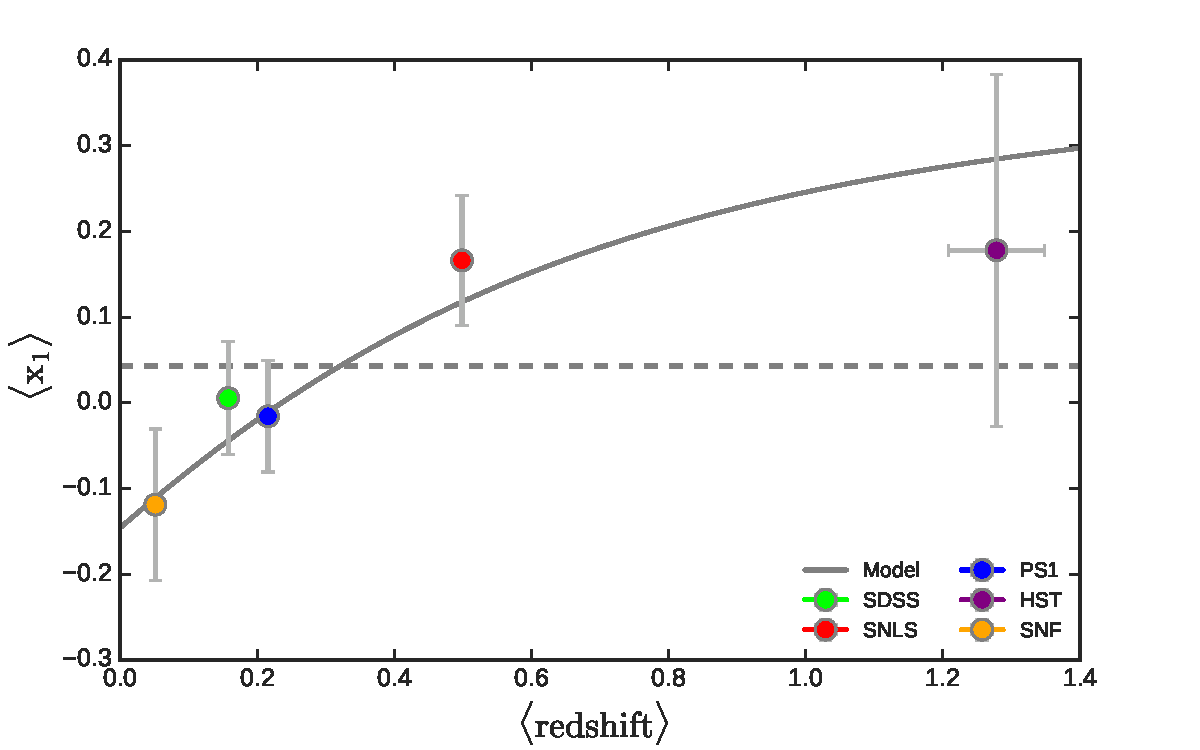
\includegraphics[width=.7\linewidth]{Rapport_figures/model_snf.pdf}
    \captionsetup{justification=centering}
    \caption{Extrapolation du modèle déterminé à partir des données de SNf sur
    la gamme de redshifts étudiés par les échantillons étudiés en gris ; moyenne
des stretchs et des redshifts des échantillons respectivement en ordonnée et en
abscisse.}
    \label{fig:model_snf}
\end{figure}

On remarque que plus le redshift est important, plus le stretch moyen semble
grand. Si l'on se rappelle que les SNe~Ia à faible stretch sont quasi-uniquement
des SNe~Ia vieilles (voir fig~\ref{fig:snf_data}) et que la fraction de veilles
SNe~Ia diminue avec le redshift (pour la gamme de redshift couvert par les
SNe~Ia), alors l'évolution visible fig.~\ref{fig:model_snf} est celle à laquelle
nous nous attendions. \bigbreak

La distribution normalisée de stretch à un redshift donné $\D(x_1 | z)$ est la
somme pondérée des distributions de stretch des jeunes et des vieilles SNe~Ia
étant donné leurs fractions relatives à ce redshift. Ainsi, dans le cas du
modèle 3G2M2S$_{\mathrm{SNf}}$ et en supposant l'évolution des fractions de
jeunes SNe~Ia de \cite{rigault_strong_2018} :

\begin{equation}
    \label{eq:dist}
    \D(x_1 | z) = \de\z \times\mathcal{N}_1 + \LF{1-\de\z}\times
    \LF{a\mathcal{N}_1 + (1-a) \mathcal{N}_2}
\end{equation}

Ce modèle est entièrement prédictif et ne dispose d'aucun paramètre libre ; ils
sont tous fixés par les données de SNf. La fig.~\ref{fig:model_snf} montre que
notre modèle est particulièrement bien en accord avec les mesures issues des
données de la littérature. \bigbreak

Alternativement, nous pouvons séparer les SNe~Ia par gammes de redshift plutôt
que par échantillon d'origine. Cela est montré fig.~\ref{fig:3G2M2S}. Nous
pouvons également ajuster l'ensemble des paramètres du modèle -- hormis les
paramètres d'évolution de la fraction de jeunes et de vieilles qui sont fixes --
non plus sur les données de SNf mais sur l'ensemble des données. Si l'on fait
ainsi, on trouve les résultats table \ref{tab:val}. Ce modèle, appelé 3G2M2S,
est illustré fig.~\ref{fig:3G2M2S} et est similaire avec celui ajusté sur les
données de SNf.

\begin{figure}[htbp!]
    \centering
    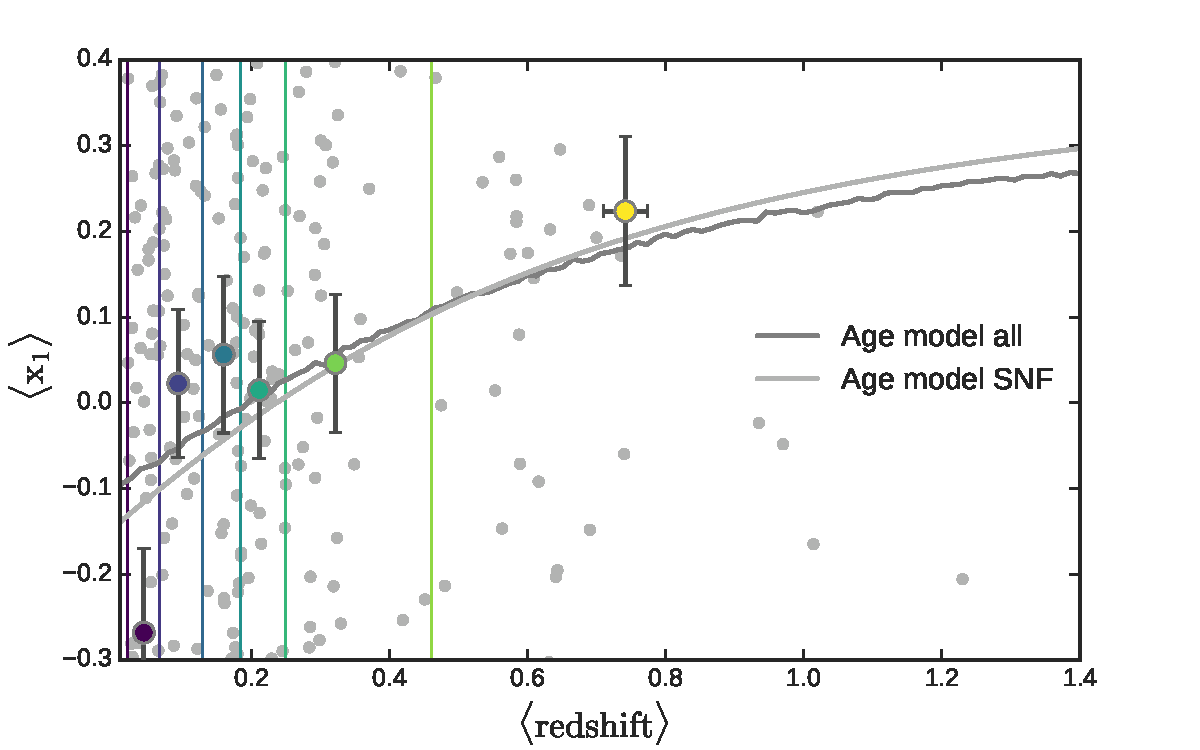
\includegraphics[width=.7\linewidth]{Rapport_figures/model_all.pdf}
    \captionsetup{justification=centering}
    \caption{Implémentation du modèle 3G2M2S en utilisant toutes les données.
    La gamme de redshifts a été divisée en 6 intervalles qui contiennent le même
nombre de données.}
    \label{fig:3G2M2S}
\end{figure}

\subsection{Modifications et comparaisons}\label{ssec:comp}

Le modèle que nous avons mis en place et qui est décrit eq.~\ref{eq:dist},
semble une relativement bonne description des données ; cf.
section~\ref{ssec:model}. Cependant, d'autres modèles auraient pu être
implémentés. Notamment, la question est de savoir si un modèle sans évolution
de population avec le redshift, i.e. $\de\z=\mathrm{constant}$, peut également
être une bonne représentation des données. Il s'agit là de l'hypothèse nulle de
notre analyse où l'on cherche à savoir s'il existe un évolution de la population
des SNe~Ia avec le redshift. \bigbreak

Nous avons en tout comparé dix modèles différents : quatre disposant d'une
évolution avec le redshift ($\de \z$ de \cite{rigault_strong_2018} et donné
eq.~\ref{eq:depsi}) mais ayant différentes fonctions de distributions de stretch
pour les jeunes et les vieilles SNe~Ia ; et six sans évolution avec le redshift
($\de\z=\mathrm{constant}$), et ayant différentes fonctions de distributions de
stretch. Les modèles disposant d'une évolution avec le redshift sont :

\begin{itemize}

    \item 3G2M2S, c'est le modèle décrit section~\ref{ssec:model} ; 

    \item 3G2M1S, c'est le même modèle que 3G2M2S en supposant que toutes les
        gaussiennes ont le même écart type ($\sigma_1\equiv\sigma_2$) ;

    \item 2G2M2S ou Howell, il s'agit du modèle présenté par
        \cite{howell_effect_2009} où les stretchs des SNe~Ia jeunes et vieilles
        ont chacun leur propre distribution gaussienne ;

    \item 3G3M3S, c'est un modèle similaire à 3G2M2S, ici encore le stretch des
        SNe~Ia jeunes est décrit par une simple distribution gaussienne et celui
        des vieilles par une double gaussienne, mais avec trois gaussiennes
        indépendantes.

\end{itemize}

Les modèles ne disposant pas d'évolution avec le redshift sont les mêmes que
ceux que l'on vient de présenter, mais dont on a forcé $\de\z=f$ où $f$ est une
constante ajustée en même temps que les autres paramètres. Nous avons également
ajouté deux autres modèles pertinents pour l'analyse :

\begin{itemize}

    \item 1G1M1S, le modèle le plus simple, la distribution de stretch des
        SNe~Ia est une simple gaussienne ;

    \item 1G1M2S ou Kessler, le modèle de distribution de stretch présenté dans
        \cite{kessler_correcting_2017}, et utilisé dans les dernières analyses
        cosmologiques \cite{scolnic_complete_2018}. Il s'agit d'un modèle de
        gaussienne asymétrique tel que :

\end{itemize}

\begin{align}
 p(x_1^i, \d x_1^i | \m, \s_-, \s_+) = 
    \begin{cases}
        \mathcal{N} \LF{\m, \sqrt{\s_-{}^2 + \d x_1^i{}^{2}}} (x_1^i) & \text{si
        } x_1^i\geq \m\\
        \mathcal{N} \LF{\m, \sqrt{\s_+{}^2 + \d x_1^i{}^{2}}} (x_1^i), &
        \text{sinon}
    \end{cases}
\end{align} 

Pour comparer les différents modèles, nous utilisons le \textit{Akaike
Information Criterion} corrigé pour des échantillons de taille finie
\cite{burnham_model_2002}. Il s'agit d'un test statistique similaire à celui du
rapport des vraisemblances, mais qui pénalise pour l'utilisation de paramètres
libres supplémentaires tel que :

\begin{equation}
    \mathrm{AICc} = \mathrm{AIC} + \LR{2k\LF{k+1}}{n - k - 1}
\end{equation}

\noindent avec $\mathrm{AIC} = 2k - 2\ln\LF{\mathcal{L}}$, où k le nombre de
paramètres libres, $\mathcal{L}$ la vraisemblance. \bigbreak

Le modèle avec le plus petit $\mathrm{AICc}$ est statistiquement considéré comme
le meilleur. Un autre modèle se compare à lui à travers son $\D \mathrm{AICc}
\equiv \mathrm{AICc_{best}}-\mathrm{AICc_{other}}$, sachant que la probabilité
que ce second modèle soit au moins aussi représentatif des données que le
meilleur modèle est donnée par :

\begin{equation}
    p(\mathrm{other} > \mathrm{best}) = \exp\LF{\D\mathrm{AICc}/2}
\end{equation}

Ainsi, un modèle avec $\abs{\D\mathrm{AICc}} < 2$ est semblable au meilleur
modèle (à $\approx1\s$) ; si $2<\abs{\D\mathrm{AICc}}<10$ il est défavorisé
($\lesssim3\s$) ; si $10<\abs{\D\mathrm{AICc}}<20$ alors il est fortement
défavorisé ($\lesssim5\s$) et si $20<\abs{\D \mathrm{AICc}}$ il est exclu. La
table \ref{tab:comp} rassemble les vraisemblances et les tests de AICc pour
l'ensemble des modèles décrits précédemment. \bigbreak

\begin{table}[htbp!]
    \centering
    \captionsetup{justification=centering}
    \caption{Comparaison des modèles. NR représente les modèles implémentés
             durant ce stage. (F) indique les modèles pour lesquels il n'y a pas
             d'évolution de la fraction de SNe~Ia jeunes et vieilles en fonction
             du redshift.}
    \label{tab:comp}
    \begin{tabularx}{\linewidth}{|Y*{6}{|Y}|}\hline

        \rowcolor{gray!15} Nom modèle & Description & Param. libres &
        $\ln\mathcal{L}$ & 
        
        $AICc$ & $\D AICc$ (from NR 1S) & Proba (from NR 1S) \\\hline\hline

        3G2M1S & NR 1S & 4 & 1815 & 1823 & 0.0 & $1.0$ \\\hline

        3G2M2S & NR 2S & 5 & 1815  & 1825 & -2.0 & $3.6\times10^{-1}$ \\\hline

        2G2M2S & Howell & 4 & 1818  & 1826 & -3.4 & $1.8\times10^{-1}$ \\\hline

        3G3M3S & NR 3S & 7 & 1812  & 1826 & -3.6 & $1.6\times10^{-1}$ \\\hline

        3G3M3SF & NR 3S (F) & 8 & 1813 & 1829 & -6.3  & $4.3\times10^{-2}$
        \\\hline

        2G2M2SF & Howell (F) & 5 & 1823  & 1833 & -9.9 & $7.0\times10^{-3}$
        \\\hline

        3G2M1SF & NR 1S (F) & 5 & 1823  & 1833 & -10.4 & $5.5\times10^{-3}$
        \\\hline

        3G2M2SF & NR 2S (F) & 6 & 1823  & 1835 & -12.0 & $2.5\times10^{-3}$
        \\\hline

        1G1M2S & Kessler (F) & 3 & 1837  & 1843 & -20.2 & $4.1\times10^{-5}$
        \\\hline

        1G1M1S & 1 gauss. (F) & 2 & 1872 & 1876 & -53.5 &
        $2.4\times10^{-12}$\\\hline

    \end{tabularx}
\end{table}

Le premier modèle mis en place section \ref{ssec:model} n'est finalement pas
celui minimisant la perte d'information. Il apparaît qu'une répartition avec un
unique écart-type soit plus représentative de la réalité (3G2M1S). Cependant,
avec un $\abs{\D\mathrm{AICc}}=2$, 3G2M1S et 3G2M2S sont comparables. Plus
généralement les modèles disposant d'une évolution de la fraction de jeune et
vieille SNe~Ia avec le redshift semblent être de bonnes représentations des
données en comparaison du meilleur modèle ($\abs{\D\mathrm{AICc}}<5$). Par
contre, ceux n'en disposant pas, ceux avec un (F) table~\ref{tab:comp}, sont
systématiquement les plus mauvais. Leur $\abs{\D\mathrm{AICc}}$ est supérieur à
5, et ils sont donc défavorisés, voire même exclus pour le modèle de
\cite{kessler_correcting_2017} ou celui de la simple gaussienne. \bigbreak

D'après nos données, il est donc fortement probable qu'il existe une évolution
de la distribution de stretch des SNe~Ia en fonction du redshift induite par une
évolution d'âge du progéniteur comme suggéré par \cite{howell_effect_2009,
rigault_evidence_2013, rigault_strong_2018}.

\section{Conclusion et perspectives}\label{sec:conc}

L'utilisation des SNe~Ia en cosmologie repose sur le fait qu'elles soient des
chandelles standardisables, c'est-à-dire qu'avec un nombre limité de paramètres,
nous soyons capable de déterminer leur luminosité. Ces paramètres sont issus de
leurs courbes de lumières. Le temps d'évolution de cette courbe, appelé stretch,
est un des deux paramètres fondamentaux. Il est directement relié à la physique,
encore largement inconnue, de l'explosion du progéniteur en SNe~Ia. Cette
méconnaissance est aujourd'hui un facteur limitant pour les analyses
cosmologiques car elle questionne notre capacité à prédire correctement la
magnitude des SNe~Ia à n'importe quel redshift. \bigbreak

Dans ce stage nous avons utilisé la distribution de stretch de données de la
littérature pour tester si celle-ci évoluait en fonction du redshift, ce qui
serait une preuve que la physique des SNe~Ia elle-même en dépend. Après avoir
construit un sous-échantillon à partir de ces données pour en extraire un
dépourvu d'effets de sélection --~effets qui auraient faussés nos mesures~--,
nous avons modélisé l'évolution du stretch des SNe~Ia en fonction du redshift.
Plusieurs formes de distributions ont été testées mais celles-ci peuvent se
ranger en deux catégories : celles disposant d'une évolution de la fraction de
jeunes et vieilles SNe~Ia en fonction du redshift, et celles n'en disposant pas.
En s'appuyant sur le test statistique AICc, nous avons déterminé qu'il est
fortement probable qu'il existe une évolution de la distribution de stretch des
SNe~Ia en fonction du redshift induite par une évolution d'âge du progéniteur
comme suggéré. Nous avons également exclu que le modèle actuellement utilisé en
cosmologie pour décrire la distribution de stretch des SNe~Ia (sans évolution de
redshift) soit une représentation correcte des données. Un article décrivant nos
travaux est en cours de rédaction et devrait etre rapidement soumis au journal
européen Astronomy \& Astrophysics. \bigbreak

Dans le futur, nous allons améliorer la construction de l'échantillon d'étude,
notamment en travayant sur les conséquences du changement du redshift limite
des échantillons publics sur nos résultats. Mais surtout, nous allons nous
intéresser aux conséquences de nos travaux sur la détermination des paramètres
cosmologiques. Il s'agira là du début de mon travail de thèse.

%\bibliographystyle{siam}
%\bibliography{VIDSTIA.bib}

\bibliographystyle{aa}
\begin{thebibliography}{23}
\expandafter\ifx\csname natexlab\endcsname\relax\def\natexlab#1{#1}\fi

\bibitem[{\bsc{Astier} et al.(2006)}]{astier_supernova_2006}
{\em The {Supernova} {Legacy} {Survey}: {Measurement} of $\O_m$, $\O_\L$ and $w$
from the {First} {Year} {Data} {Set}}, Astier, P. , Guy, J. et~al. 2006,
Astronomy \& Astrophysics, 447, 31, arXiv: astro-ph/0510447

\bibitem[{\bsc{Betoule} et al.(2014)}]{betoule_improved_2014}
{\em Improved cosmological constraints from a joint analysis of the {SDSS}-{II}
and {SNLS} supernova samples}, Betoule, M., Kessler, R. et~al. 2014, Astronomy
and Astrophysics, 568, A22

\bibitem[{\bsc{Burnham} et al.(2002)}]{burnham_model_2002}
{\em Model Selection and Multimodel Inference: A Practical Information-Theoretic
Approach}, K.~P. Burnham and D.~R. Anderson, Springer-Verlag, 2~ed.

\bibitem[{\bsc{Childress} {et~al.}(2014)}]{childress_ages_2014}
{\em Ages of {Type} {Ia} supernovae over cosmic time} Childress, M.~J., Wolf,
C., \& Zahid, H.~J. 2014, Monthly Notices of the Royal Astronomical Society,
445, 1898

\bibitem[{\bsc{Guy} et al.(2007)}]{guy_salt2_2007}
{\em {SALT}2: using distant supernovae to improve the use of type {Ia}
supernovae as distance indicators}, Guy, J., Astier, P. et~al. 2007, Astronomy
and Astrophysics, 466, 11

\bibitem[{\bsc{Guy} et al.(2010)}]{guy_supernova_2010}
{\em The {Supernova} {Legacy} {Survey} 3-year sample: {Type} {Ia} supernovae
photometric distances and cosmological constraints}, Guy, J., Sullivan, M.
et~al. 2010, Astronomy and Astrophysics, 523, A7

\bibitem[{\bsc{Howell} et al.(2007)}]{howell_predicted_2007}
{\em Predicted and Observed Evolution in the Mean Properties of Type Ia
Supernovae with Redshift}, D.~A. Howell, M.~Sullivan et~al. 2009, The
Astrophysical Journal, 667, p.~L37.

\bibitem[{\bsc{Howell} et al.(2009)}]{howell_effect_2009}
{\em The {Effect} of {Progenitor} {Age} and {Metallicity} on {Luminosity} and
$^{56}${Ni} {Yield} in {Type} {Ia} {Supernovae}}, Howell, D.~A., Sullivan, M.
et~al. 2009, The Astrophysical Journal, 691, 661

\bibitem[{\bsc{Kessler} et al.(2017)}]{kessler_correcting_2017}
{\em Correcting {Type} {Ia} {Supernova} {Distances} for {Selection} {Biases} and
{Contamination} in {Photometrically} {Identified} {Samples}}, R.~Kessler and
D.~Scolnic, The Astrophysical Journal, 836 (2017), p.~56.

\bibitem[{\bsc{Madau} et al.(2014)}]{madau_cosmic_2014}
{\em Cosmic {Star} {Formation} {History}}, Madau, P., Dickinson, M. 2014, Annual
Review of Astronomy and Astrophysics, 52, 415, arXiv: 1403.0007

\bibitem[{\bsc{Mannucci} et al.(2005)}]{mannucci_supernova_2005}
{\em The supernova rate per unit mass}, Mannucci, F., Della~Valle, M. et~al.
2005, Astronomy and Astrophysics, 433, 807

\bibitem[{\bsc{Pereira} et al.(2013)}]{pereira_spectrophotometric_2013}
{\em Spectrophotometric time series of {SN} 2011fe from the {Nearby} {Supernova}
{Factory}}, Pereira, R., Thomas, R. C. et~al. 2013, Astronomy and Astrophysics,
554, A27

\bibitem[{\bsc{Perlmutter} et al.(1999)}]{perlmutter_measurements_1999}
{\em Measurements of {Omega} and {Lambda} from 42 {High}-{Redshift}
{Supernovae}}, Perlmutter, S., Aldering, G. et~al. 1999, The Astrophysical
Journal, 517, 565, arXiv: astro-ph/9812133

\bibitem[{\bsc{Phillips}(1999)}]{phillips_absolute_1999}
{\em The {Absolute} {Magnitudes} of {Type} {IA} {Supernovae} - {NASA}/{ADS}},
Phillips, M.~M. 1999, Astrophysical Journal Letters, v.413, p.L105

\bibitem[{\bsc{Riess} et al.(1998)}]{riess_observational_1998}
{\em Observational {Evidence} from {Supernovae} for an {Accelerating} {Universe}
and a {Cosmological} {Constant}}, Riess, A.~G., Filippenko, A. V. et~al. 1998,
The Astronomical Journal, 116, 1009, arXiv: astro-ph/9805201

\bibitem[{\bsc{Riess} \& \bsc{Livio}(2006)}]{riess_first_2006}
{\em The {First} {Type} {Ia} {Supernovae}: {An} {Empirical} {Approach} to
{Taming} {Evolutionary} {Effects} in {Dark} {Energy} {Surveys} from {SNe} {Ia}
at z>2}, Riess, A.~G. \& Livio, M. 2006, The Astrophysical Journal, 648, 884

\bibitem[{\bsc{Rigault} et al.(2015)}]{rigault_confirmation_2015}
{\em Confirmation of a {Star} {Formation} {Bias} in {Type} {Ia} {Supernova}
{Distances} and its {Effect} on the {Measurement} of the {Hubble} {Constant}},
Rigault, M., Aldering, G. et~al. 2015, The Astrophysical Journal, 802, 20

\bibitem[{\bsc{Rigault} et al.(2018)}]{rigault_strong_2018}
{\em Strong {Dependence} of {Type} {Ia} {Supernova} {Standardization} on the
{Local} {Specific} {Star} {Formation} {Rate}}, Rigault, M., Brinnel, V. et~al.
2018, arXiv e-prints, arXiv:1806.03849

\bibitem[{\bsc{Rigault} et al.(2013)}]{rigault_evidence_2013}
{\em Evidence of environmental dependencies of {Type} {Ia} supernovae from the
{Nearby} {Supernova} {Factory} indicated by local {H}$\alpha$}, Rigault, M.,
Copin, Y. et~al. 2013, Astronomy and Astrophysics, 560, A66

\bibitem[{\bsc{Scannapieco} \& \bsc{Bildsten}(2005)}]{scannapieco_type_2005}
{\em The {Type} {Ia} {Supernova} {Rate}}, Scannapieco, E. \& Bildsten, L. 2005,
The Astrophysical Journal, 629, L85

\bibitem[{\bsc{Scolnic} et al.(2018)}]{scolnic_complete_2018}
{\em The {Complete} {Light}-curve {Sample} of {Spectroscopically} {Confirmed}
{SNe} {Ia} from {Pan}-{STARRS}1 and {Cosmological} {Constraints} from the
{Combined} {Pantheon} {Sample}}, Scolnic, D.~M., Jones, D. O. et~al. 2018, The
Astrophysical Journal, 859, 101

\bibitem[{\bsc{Sullivan} et al.(2010)}]{sullivan_dependence_2010}
{\em The dependence of {Type} {Ia} {Supernovae} luminosities on their host
galaxies}, Sullivan, M., Conley, A. et~al. 2010, Monthly Notices of the Royal
Astronomical Society, 406, 782

\bibitem[{\bsc{Sullivan} et al.(2006)}]{sullivan_rates_2006}
{\em Rates and {Properties} of {Type} {Ia} {Supernovae} as a {Function} of
{Mass} and {Star} {Formation} in {Their} {Host} {Galaxies}}, Sullivan, M.,
Le~Borgne, D. et~al. 2006, The Astrophysical Journal, 648, 868

\bibitem[{\bsc{Tasca} et al.(2015)}]{tasca_evolving_2015}
{\em The evolving star formation rate: {M}$_\star$ relation and {sSFR} since z ≃
5 from the {VUDS} spectroscopic survey}, Tasca, L. a.~M., Le~Fèvre, O. et~al.
2015, Astronomy and Astrophysics, 581, A54

\bibitem[{\bsc{Tripp}(1998)}]{tripp_two-parameter_1998}
{\em A two-parameter luminosity correction for {Type} {IA} supernovae}, Tripp,
R. 1998, Astronomy and Astrophysics, 331, 815

\bibitem[{\bsc{Wood-Vasey} et al.(2004)}]{wood-vasey_nearby_2004}
{\em The {Nearby} {Supernova} {Factory}}, Wood-Vasey, W.~M., Aldering, G. et~al.
2004, New Astronomy Reviews, 48, 637, arXiv: astro-ph/0401513

\end{thebibliography}
\addcontentsline{toc}{section}{Bibliographie}
\end{document}end{document}
